\documentclass[aspectratio=169,11pt]{beamer}
\usepackage{amsmath,amssymb,mathtools,lmodern,booktabs,tikz}
\usefonttheme{professionalfonts}
\definecolor{navy}{HTML}{192D44}
\definecolor{teal}{HTML}{197584}
\definecolor{pale}{HTML}{EAF2F6}
\setbeamercolor{normal text}{fg=navy,bg=white}
\setbeamercolor{frametitle}{fg=white,bg=navy}
\setbeamercolor{block title}{fg=teal,bg=pale}
\setbeamercolor{block body}{fg=navy,bg=pale}
\setbeamerfont{frametitle}{family=\rmfamily,series=\bfseries,size=\fontsize{12}{14}\selectfont}
\setbeamertemplate{navigation symbols}{}
\setbeamertemplate{frametitle}{\nointerlineskip\begin{beamercolorbox}[wd=\paperwidth,ht=.60cm,dp=.26cm,leftskip=.3cm]{frametitle}\insertframetitle\end{beamercolorbox}}
\setbeamersize{text margin left=1cm,text margin right=1cm}
\setbeamertemplate{footline}{\hspace{1cm}\color{navy!65}\fontsize{8}{10}\selectfont\insertsectionhead\hfill\insertframenumber\ /\ \inserttotalframenumber\hspace{1cm}\vspace{5pt}}
\setlength{\parskip}{5pt}
\newcommand{\Z}{\mathbb Z}
\newcommand{\R}{\mathbb R}
\newcommand{\C}{\mathbb C}
\newcommand{\F}{\mathbb F}
\newcommand{\N}{\mathbb N}
\newcommand{\ind}{\mathbf1}
\newcommand{\dd}{\,\mathrm d}
\newcommand{\HW}[2]{{\color{teal}\textbf{Homework #1, Problem #2.}}}
\newcommand{\link}[2]{{\color{teal}\href{#1}{#2}}}
\newcommand{\oaurl}{https://github.com/openai/math/blob/main/preprints/Uniform-exclusion-of-Landau-Siegel-zeros-October-1-2026/paper.pdf}
\hypersetup{pdftitle={MATH 8440: Complete course notes},pdfauthor={Paul Pollack}}
\begin{document}

% ---- sections/01-infinitude ----
\begingroup
\setbeamercolor{background canvas}{bg=navy}
\setbeamertemplate{frametitle}{}
\setbeamertemplate{footline}{}
\begin{frame}[plain,t]{}
\color{white}
\vspace{.6cm}
{\color[HTML]{DFB86D}\large MATH 8440\quad/\quad FALL 2026}\par
Topics in Analytic and Combinatorial Number Theory\par
\vspace{.85cm}
{\rmfamily\fontsize{27}{32}\selectfont Elementary methods in the\\distribution of prime numbers\par}
\vspace{.65cm}
{\color[HTML]{DFB86D}\rule{2.6cm}{.7pt}}\par
\vspace{.5cm}
Paul Pollack\par
University of Georgia
\end{frame}
\endgroup
\begin{frame}[label=overview]{The course at a glance}
\small
\textbf{Infinitely many primes.} Euclid, Euler, squarefree integers, and two proofs from algebra.

\textbf{Prime-producing sequences.} Euler's quadratic and an example of Erd\H{o}s.

\textbf{Counting primes.} Chebyshev's bounds and Bertrand's postulate.

\textbf{Mertens' estimates.} Prime sums, products, and guesses about primes.

\textbf{Primes in progressions.} Schur's lemma and the classes $1$ and $-1$.

\textbf{Dirichlet's theorem.} Characters and the values $L(1,\chi)$.

\textbf{The prime number theorem.} M\"obius sums, smooth numbers, and the hyperbola method. \textbf{Bonus:} $\sum\mu(n)/n=0$.
\end{frame}
\section{Infinitely many primes}

% ---- sections/toc-003 ----
\begin{frame}{Infinitely many primes (1 of 3)}
\small\renewcommand{\arraystretch}{1.35}
\begin{tabular}{p{.79\textwidth}r}\textbf{Contents}&\textbf{Pages}\\\midrule
\hyperlink{Navigation6}{Euclid's proof}&6\\
\hyperlink{Navigation7}{The proofs of Stieltjes and Braun}&7--8\\
\hyperlink{Navigation9}{Euclid's lemma}&9\\
\hyperlink{Navigation10}{Furstenberg's proof}&10--11\\
\hyperlink{Navigation12}{Goldbach's proof and the Fermat numbers}&12--13\\
\hyperlink{Navigation14}{Prime factors of $2^p-1$}&14\\
\hyperlink{Navigation15}{Multiplicative functions}&15\\
\hyperlink{Navigation16}{Euler's factorization theorem}&16--17\\
\end{tabular}\par\medskip\hyperlink{overview}{\color{teal}Course overview}\end{frame}


% ---- sections/toc-004 ----
\begin{frame}{Infinitely many primes (2 of 3)}
\small\renewcommand{\arraystretch}{1.35}
\begin{tabular}{p{.79\textwidth}r}\textbf{Contents}&\textbf{Pages}\\\midrule
\hyperlink{Navigation18}{Euler's proof that $\sum_p1/p$ diverges}&18\\
\hyperlink{Navigation19}{Upper and lower bounds for $\sum_{p\le x}1/p$}&19--20\\
\hyperlink{Navigation21}{Hacks's proof using $\zeta(2)$}&21\\
\hyperlink{Navigation22}{Infinitude from $\zeta(2)^2/\zeta(4)$}&22\\
\hyperlink{Navigation23}{Exercises on Euler products}&23\\
\hyperlink{Navigation24}{Perott's proof using squarefree integers}&24\\
\hyperlink{Navigation25}{Erd\H{o}s's lower bound for $\pi(N)$}&25\\
\hyperlink{Navigation26}{Erd\H{o}s's proof that $\sum_p1/p$ diverges}&26\\
\end{tabular}\par\medskip\hyperlink{overview}{\color{teal}Course overview}\end{frame}


% ---- sections/toc-005 ----
\begin{frame}{Infinitely many primes (3 of 3)}
\small\renewcommand{\arraystretch}{1.35}
\begin{tabular}{p{.79\textwidth}r}\textbf{Contents}&\textbf{Pages}\\\midrule
\hyperlink{Navigation27}{The identity $\sum_{d\mid n}\mu(d)=\ind_{n=1}$}&27\\
\hyperlink{Navigation28}{Infinitude from the support of $\mu$}&28\\
\hyperlink{Navigation29}{M\"obius inversion}&29--30\\
\hyperlink{Navigation31}{Counting smooth integers}&31--33\\
\hyperlink{Navigation34}{The maximal ideals of $\Z[X]$}&34--35\\
\hyperlink{Navigation36}{Washington's proof}&36--37\\
\end{tabular}\par\medskip\hyperlink{overview}{\color{teal}Course overview}\end{frame}

\begin{frame}{Euclid's proof}
A prime is an integer greater than $1$ whose only positive divisors are $1$ and itself. Here are the first few:
\[2,\quad3,\quad5,\quad7,\quad11,\quad13,\quad17.\]
Let $p_1,\ldots,p_k$ be any finite list of distinct primes, and put $P=p_1\cdots p_k$. Look at $P+1$. We know $P+1>1$, so $P+1$ has some prime factor $q$. But $P+1\equiv1\pmod{p_i}$ for all $i$, and so $q\notin\{p_1,\ldots,p_k\}$. So there must be infinitely many primes.
\end{frame}
\begin{frame}{The proof of Stieltjes}
\textbf{Stieltjes.} Factor $P=AB$ with $A,B>0$. Each $p_i$ divides exactly one of $A,B$, so it cannot divide $A+B$. Take any prime factor of $A+B$. Choosing $B=1$ gives Euclid's proof.
\end{frame}
\begin{frame}{The proof of Braun}
\textbf{Braun.} Suppose $k\ge2$. Put the fractions over a common denominator:
\[\frac1{p_1}+\cdots+\frac1{p_k}=\frac NP,\qquad N=\frac P{p_1}+\cdots+\frac P{p_k}.\]
For each $i$, $p_i$ divides $P/p_j$ for all $j\ne i$. Thus $N\equiv P/p_i\pmod{p_i}$. If $p_i\mid N$, then $p_i\mid P/p_i$ and $p_i^2\mid P$, a contradiction. Take any prime $q\mid N$. (This proof needs $k\ge2$.)

Another variant is to look at $m!+1$. Every prime factor exceeds $m$.
\end{frame}
\begin{frame}{Euclid's lemma}
\HW{1}{2} Here is a slightly unusual proof of Euclid's lemma. Fix a prime $p$ and an integer $a$, and consider $I=\{b\in\Z:p\mid ab\}$. The difference of two members of $I$ again belongs to $I$, as does every integer multiple of a member of $I$. Thus $I$ is an ideal of $\Z$.

Write $I=d\Z$ with $d>0$ (notice that $p\in I$). Then $d\mid p$, so either $d=1$ or $d=p$. If $d=1$, then $1\in I$, whence $p\mid a$. If $d=p$, then every $b$ for which $p\mid ab$ is itself divisible by $p$. These are precisely the two alternatives in Euclid's lemma.
\end{frame}
\begin{frame}{Furstenberg's proof}
For $m>0$ let
\[U_{a,m}=\{n\in\Z:n\equiv a\pmod m\}.\]
The \emph{profinite topology} is the topology on $\Z$ with basic open sets $U_{a,m}$. To check that this makes sense, observe that these sets cover $\Z$. If $n$ belongs to two of them, the progression through $n$ modulo the product of their moduli lies in both (Homework 1, Problem 1).

Each set $U_{a,m}$ is closed. Indeed, its complement is the union of the other classes modulo $m$. Also, every nonempty open set is infinite, since it contains a full arithmetic progression.
\end{frame}
\begin{frame}{Furstenberg's proof}
Suppose $p_1,\ldots,p_k$ are all the primes. The set of integers divisible by at least one of them is
\[U_{0,p_1}\cup\cdots\cup U_{0,p_k}.\]
This set is closed (a finite union of closed sets). Hence its complement is open. But the complement consists of the integers divisible by no prime, namely $\{-1,1\}$. This is a contradiction, since nonempty open sets are infinite.
\end{frame}
\begin{frame}{Goldbach's proof and the Fermat numbers}
Suppose $a_1,a_2,\ldots$ is an infinite sequence of integers greater than $1$, with $(a_i,a_j)=1$ whenever $j<i$. Let $p_i$ be a prime factor of $a_i$. Then $p_1,p_2,\ldots$ is an infinite sequence of distinct primes.

How do we get such a sequence? Goldbach takes $a_1=3$, and for $i>1$ sets
\[a_i=2+\prod_{1\le j<i}a_j.\]
First, notice that each $a_i$ is odd, by induction. If $d\mid a_i$ and $d\mid a_j$, where $j<i$, then $d\mid a_j\mid a_i-2$. Thus $d\mid2$; since $a_i$ is odd, $d=1$.

The sequence begins $3,5,17,257,65537$. This suggests $a_i=2^{2^{i-1}}+1$.
\end{frame}
\begin{frame}{Goldbach's proof and the Fermat numbers}
\small
Write $F_n=2^{2^n}+1$ for the $n$th Fermat number. Factoring a difference of squares repeatedly gives
\[F_n-2=2^{2^n}-1=(2^{2^{n-1}}+1)(2^{2^{n-1}}-1)=F_{n-1}\cdots F_0\quad(n\ge1).\]
Thus $a_i=F_{i-1}$. We do not need the Fermat numbers themselves to be prime. Indeed, $F_5=641\cdot6700417$.

If $p\mid F_n$, then $2^{2^n}\equiv-1\pmod p$. The order of $2$ modulo $p$ divides $2^{n+1}$ but does not divide $2^n$, so it equals $2^{n+1}$.

In particular $2^{n+1}\mid p-1$. Distinct $n$ give distinct prime divisors, and for each fixed $k$ infinitely many of them are $1\bmod 2^k$.

\HW{1}{3} Let $n\ge2$ and let $p$ be a prime divisor of $F_n$. Prove the stronger divisibility $2^{n+2}\mid p-1$.
\end{frame}
\begin{frame}{Infinitude of primes from the factors of $2^p-1$}
Suppose there is a largest prime $p$. Let $q$ be any prime factor of $2^p-1$. Then
\[2^p\equiv1\pmod q.\]
Hence the order of $2$ modulo $q$ divides $p$. The order is not $1$, since $q\nmid2-1$. It follows that the order is $p$. By Lagrange's theorem, $p\mid q-1$. Hence $q>p$, contrary to the choice of $p$.
\end{frame}
\begin{frame}{Multiplicative functions}
An arithmetic function is a function on the positive integers. We call $f$ \emph{multiplicative} if $f(1)=1$ and $f(ab)=f(a)f(b)$ whenever $(a,b)=1$. Hence
\[f(p_1^{e_1}\cdots p_k^{e_k})=\prod_{i=1}^k f(p_i^{e_i})\]
whenever the $p_i$ are distinct. Conversely, this identity implies multiplicativity (Homework 1, Problem 8).

The functions $1$ and $n^s$ are examples, as is Euler's $\phi(n)=\#(\Z/n\Z)^\times$. For $\phi$, apply the Chinese remainder theorem and count units on both sides. For $\sigma(n)=\sum_{d\mid n}d$, observe that specifying a divisor amounts to choosing, independently for each $p_i$, an exponent between $0$ and $e_i$.
\end{frame}
\begin{frame}{Euler's factorization theorem}
\begin{block}{Theorem}For a multiplicative function $f$,
\[\sum_{n\ge1}f(n)=\prod_p(1+f(p)+f(p^2)+\cdots)\]
if $\sum_n|f(n)|$ converges, or if the product with $|f|$ in place of $f$ is finite.
\end{block}
Suppose first that $\sum_n|f(n)|<\infty$. On multiplying out just the factors corresponding to $p\le x$, unique factorization gives
\[\prod_{p\le x}(1+f(p)+f(p^2)+\cdots)=\sum_{\substack{n\ge1\\p\mid n\Rightarrow p\le x}}f(n).\]
\end{frame}
\begin{frame}{Euler's factorization theorem}
What have we left out? Only integers having a prime factor $>x$, all of which are themselves $>x$. Thus the error is bounded by $\sum_{n>x}|f(n)|$, which tends to zero.

Suppose now that we are given convergence of the product for $|f|$. Then
\[\sum_{n\le x}|f(n)|\le\prod_{p\le x}(1+|f(p)|+|f(p^2)|+\cdots)\le\prod_p(1+|f(p)|+|f(p^2)|+\cdots).\]
The partial sums on the left increase and are bounded. Thus the series converges absolutely, and the first argument applies.
\end{frame}
\begin{frame}{Euler's proof that $\sum_p1/p$ diverges}
What happens if we try $f(n)=1/n$? For any one prime $p$ we have
\[1+\frac1p+\frac1{p^2}+\cdots=(1-1/p)^{-1}.\]
If there were only finitely many primes, the product would be finite. Euler's theorem would then give convergence of $\sum_{n\ge1}1/n$!

In fact $\sum_p1/p$ diverges. Otherwise the partial products would again be bounded, since
\[(1-1/p)^{-1}=1+\frac1{p-1}\le1+\frac2p\le e^{2/p}.\]
The products would be bounded by $\exp(2\sum_p1/p)$, so the harmonic series would converge. This proves Euler's assertion.
\end{frame}
\begin{frame}{Upper and lower bounds for $\sum_{p\le x}1/p$}
For $x>1$ the integral test gives $\log x<\sum_{n\le x}1/n\le1+\log x$. Every term on the left occurs on multiplying out the product below, so
\[\log x<\prod_{p\le x}(1-1/p)^{-1}\le\exp\left(\sum_{p\le x}\frac1{p-1}\right).\]
Since $1/(p-1)=1/p+1/(p(p-1))$ and
\[\sum_{p\le x}\frac1{p(p-1)}\le\sum_{n\ge2}\left(\frac1{n-1}-\frac1n\right)=1,\]
taking logarithms gives $\sum_{p\le x}1/p>\log\log x-1$.
\end{frame}
\begin{frame}{Upper and lower bounds for $\sum_{p\le x}1/p$}
On squaring the sum, how often can a given integer occur as a denominator? At most twice, since $pq$ determines the unordered pair $\{p,q\}$. Hence
\[\left(\sum_{p\le x}\frac1p\right)^2=\sum_{p,q\le x}\frac1{pq}\le2\sum_{n\le x^2}\frac1n\le2+4\log x.\]
Already we see that the sum of the reciprocals of the primes grows more slowly than the harmonic sum.

\HW{1}{11} Take higher powers of $\sum_{p\le x}1/p$. By letting the exponent depend on $x$, prove that this sum is at most $\log\log x+O(\log\log\log x)$.
\end{frame}
\begin{frame}{Hacks's proof using $\zeta(2)$}
For $s>1$, put $\zeta(s)=\sum_{n\ge1}n^{-s}$. Euler's factorization gives
\[\zeta(s)=\prod_p(1-p^{-s})^{-1}.\]
At $s=2$ the series equals $\pi^2/6$. Recall Euler's calculation: in the sine product
\[\frac{\sin t}t=\prod_{n\ge1}\left(1-\frac{t^2}{n^2\pi^2}\right)\]
the coefficient of $t^2$ is $-\zeta(2)/\pi^2$. Comparing this with $-1/3!$ gives Euler's evaluation. If there were only finitely many primes, then $\pi^2/6$ would be a finite product of rational numbers. But $\pi^2/6$ is irrational (Homework 1, Problem 13).
\end{frame}
\begin{frame}{Infinitude of primes from $\zeta(2)^2/\zeta(4)$}
Comparing the coefficients of $t^4$ gives $(\zeta(2)^2-\zeta(4))/(2\pi^4)=1/5!$. Thus $\zeta(4)=\pi^4/90$, and
\[\frac52=\frac{\zeta(2)^2}{\zeta(4)}=\prod_p\frac{1-p^{-4}}{(1-p^{-2})^2}=\prod_p\frac{p^2+1}{p^2-1}.\]
The quotient $5/2$ is rational, so irrationality is of no help. But look at the denominator of the first factor, $5/3$. If there were only finitely many factors, some numerator $p^2+1$ would have to be divisible by $3$. But $-1$ is not a square modulo $3$, since the only squares are $0$ and $1$. This contradiction proves infinitude.
\end{frame}
\begin{frame}{Exercises on Euler products}
\HW{1}{10} Let $\chi$ be zero on even integers, $1$ on $1\bmod4$, and $-1$ on $3\bmod4$. Show that $\chi$ is completely multiplicative. Assuming there are only finitely many primes, show that
\[1-\frac13+\frac15-\frac17+\cdots=\prod_p(1-\chi(p)/p)^{-1}.\]
Use the value of the alternating series to reach a contradiction.

\HW{2}{3} Let $\mathcal P$ be the set of primes dividing at least one Fermat number. Prove that $\sum_{p\in\mathcal P}1/p$ converges. Use the order of $2$ modulo $p$ to count divisors of the higher-index Fermat numbers, and their sizes for the lower indices.
\end{frame}
\begin{frame}{Perott's proof using squarefree integers}
A positive integer is \emph{squarefree} if it is divisible by no square greater than $1$. It is determined by its set of prime divisors. With only $k$ primes there would be only $2^k$ squarefree integers.

How many $n\le N$ fail to be squarefree? At most
\[\sum_{m=2}^{\lfloor\sqrt N\rfloor}\left\lfloor\frac N{m^2}\right\rfloor\le N\sum_{m\ge2}\frac1{m^2}=cN.\]
Since $c<\int_1^\infty t^{-2}\dd t=1$, at least $(1-c)N$ integers up to $N$ are squarefree. For $N$ large this is more than $2^k$, however large we took $k$.
\end{frame}
\begin{frame}{Erd\H{o}s's lower bound for $\pi(N)$}
Every positive integer $n$ can be written uniquely as $uv^2$, with $u$ squarefree. Throw into $u$ those primes appearing to an odd power in $n$.

Let $\pi(N)=\#\{p\le N\}$. If $n\le N$, there are at most $2^{\pi(N)}$ choices for $u$, since $u$ is determined by its prime factors. There are at most $\sqrt N$ choices for $v$. Hence
\[N\le2^{\pi(N)}\sqrt N,\qquad \pi(N)\ge\frac{\log N}{\log4}.\]
So Erd\H{o}s's argument does a little more than prove infinitude. It gives a lower bound for $\pi(N)$ that tends to infinity with $N$.
\end{frame}


% ---- sections/01b-infinitude ----
\begin{frame}{Erd\H{o}s's proof that $\sum_p1/p$ diverges}
Suppose $\sum_p1/p$ converges. Choose $y$ so that $\sum_{p>y}1/p<1/2$.

How many $n\le N$ have all their prime factors at most $y$? Writing $n=uv^2$ as before gives at most $2^{\pi(y)}\sqrt N$ possibilities.

Every remaining $n$ is a multiple of a prime $p>y$. There are at most
\[\sum_{y<p\le N}\left\lfloor\frac Np\right\rfloor\le N\sum_{p>y}\frac1p<N/2\]
such multiples. We conclude that $N/2\le2^{\pi(y)}\sqrt N$. But $y$ has been fixed all along, and this fails for all sufficiently large $N$.
\end{frame}
\begin{frame}{The identity $\sum_{d\mid n}\mu(d)=\ind_{n=1}$}
Put $\mu(1)=1$, put $\mu(n)=0$ if $n$ is not squarefree, and put $\mu(n)=(-1)^k$ if $n$ is a product of $k$ distinct primes.

For $n>1$ with $k$ distinct prime factors, only products of subsets of those primes contribute. Thus
\[\sum_{d\mid n}\mu(d)=\sum_{j=0}^k(-1)^j\binom kj=(1-1)^k=0.\]
For $n=1$ we get $1$, the contribution of the empty set of primes. Thus the single formula $\sum_{d\mid n}\mu(d)=\ind_{n=1}$ covers both cases.
\end{frame}
\begin{frame}{Infinitude of primes from the support of $\mu$}
Suppose $g(n)=\sum_{d\mid n}f(d)$ and both $f$ and $g$ vanish beyond some point. We claim $f$ is identically zero.

Otherwise let $D$ be the largest index with $f(D)\ne0$. For $|z|<1$,
\[\sum_{n\ge1}g(n)z^n=\sum_{d\le D}f(d)\sum_{j\ge1}z^{dj}=\sum_{d\le D}f(d)\frac{z^d}{1-z^d}.\]
The left side is a polynomial. Let $z$ tend radially to a primitive $D$th root of unity. The $d=D$ term becomes unbounded, while every $d<D$ term has a finite limit. This proves the claim.

Take $f=\mu$ and $g=\ind_{n=1}$. Finitely many primes would mean finitely many squarefree numbers, giving $\mu=0$, although $\mu(1)=1$.
\end{frame}
\begin{frame}{M\"obius inversion}
We can regard $\sum_{n\ge1}a_nn^{-s}$ as a formal series. What matters is the coefficient of each $n^{-s}$. Since $d^{-s}e^{-s}=(de)^{-s}$,
\[\left(\sum_{d\ge1}\frac{a_d}{d^s}\right)\left(\sum_{e\ge1}\frac{b_e}{e^s}\right)=\sum_{n\ge1}\frac1{n^s}\sum_{de=n}a_db_e.\]
For example, $\zeta(s)^2=\sum_{n\ge1}\tau(n)n^{-s}$, where $\tau(n)=\#\{d:d\mid n\}$. The coefficient in $\zeta(s)^k$ counts ordered $k$-tuples with product $n$.

Each coefficient is a finite sum. We are not asserting convergence for any value of $s$.

\HW{1}{12} Consider formal Dirichlet series with complex coefficients, with termwise addition and the multiplication above. Prove that this ring is an integral domain and determine its units.
\end{frame}
\begin{frame}{M\"obius inversion}
The partial Euler product for $\zeta(s)$ over $p\le N$ has the right coefficient for every $n\le N$. Formal convergence means that each coefficient is eventually constant.
\[\zeta(s)^{-1}=\prod_p(1-p^{-s})=\sum_{n\ge1}\frac{\mu(n)}{n^s}.\]
We select $-p^{-s}$ for each $p\mid n$, so $n$ must be squarefree and its coefficient is $(-1)^{\#\{p:p\mid n\}}$.

If $g(n)=\sum_{d\mid n}f(d)$, its series is $\zeta(s)\sum f(n)n^{-s}$. Multiply by $1/\zeta(s)$ and compare coefficients:
\[f(n)=\sum_{d\mid n}\mu(d)g(n/d).\]
Multiplying back by $\zeta(s)$ proves the converse. This is M\"obius inversion.
\end{frame}
\begin{frame}{Infinitude of primes by counting smooth integers}
Call $n$ \emph{$y$-smooth} if every prime factor is at most $y$. Write $\Psi(x,y)$ for their count up to $x$, including $1$.

For $y=2$ we get $1+\lfloor\log x/\log2\rfloor$. For $y=3$ count nonnegative integer pairs $(a,b)$ with
\[a\log2+b\log3\le\log x.\]
Denote by $\Delta(t)$ the triangle with $t$ on the right. Draw a unit square with lower left corner at each lattice point counted. These squares cover $\Delta(\log x)$ (round coordinates down). Increasing both coordinates by $1$ adds only $\log6$, so every square is contained in $\Delta(\log x+\log6)$.
\end{frame}
\begin{frame}{Infinitude of primes by counting smooth integers}
\begin{columns}
\column{.49\textwidth}
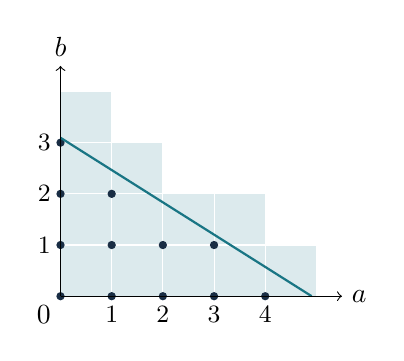
\begin{tikzpicture}[x=.65cm,y=.65cm]
\foreach \a/\b in {0/0,1/0,2/0,3/0,4/0,0/1,1/1,2/1,3/1,0/2,1/2,0/3}{\fill[teal!15] (\a,\b) rectangle +(1,1);\draw[white] (\a,\b) rectangle +(1,1);\fill[navy] (\a,\b) circle(1.5pt);}
\draw[teal,thick] (0,3.096) -- (4.907,0);
\draw[->] (0,0)--(5.5,0) node[right]{$a$};\draw[->] (0,0)--(0,4.5) node[above]{$b$};
\foreach \x in {1,2,3,4}{\node[below] at(\x,0){\small\x};}\foreach \y in {1,2,3}{\node[left] at(0,\y){\small\y};}
\node[below left] at(0,0){$0$};
\end{tikzpicture}
\column{.49\textwidth}
Each dot represents one integer $2^a3^b\le30$. For instance, $(3,1)$ represents $24$. The next dot in that column would represent $72$.

The shaded squares cover the triangle $a\log2+b\log3\le\log30$ in the first quadrant. Each has area $1$, so their combined area is $\Psi(30,3)$.
\end{columns}
\end{frame}
\begin{frame}{Infinitude of primes by counting smooth integers}
The area of $\Delta(t)$ is $t^2/(2\log2\log3)$. The two areas differ by $O(\log x)$, so
\[\Psi(x,3)=\frac{(\log x)^2}{2\log2\log3}+O(\log x).\]
For the first $k$ primes, draw unit cubes in $k$ dimensions. Their union contains the simplex with $t=\log x$ and lies in the one with $t=\log x+\sum_i\log p_i$. Changing $u_i$ to $u_i\log p_i$ gives volume $t^k/(k!\prod_i\log p_i)$. Thus
\[\Psi(x,p_k)=\frac{(\log x)^k}{k!\prod_{i=1}^k\log p_i}+O_k((\log x)^{k-1}).\]
If $p_k$ were the last prime, $\Psi(x,p_k)=\lfloor x\rfloor$. But $\Psi(x,p_k)/x\to0$, whereas $\lfloor x\rfloor/x\to1$. This proves infinitude.
\end{frame}
\begin{frame}{Infinitude of primes from the maximal ideals of $\Z[X]$}
Suppose $(f)$ is maximal. Then $\Z[X]/(f)$ is a field. A constant $f$ will not do: $f=0,\pm1$ gives $\Z[X]$ or the zero ring; for $|f|>1$ the class of $X$ is a nonzero nonunit.

If $\deg f>0$, choose an integer $n$ with $|f(n)|>1$. The constant $f(n)$ has nonzero class modulo $f(X)$. If it had an inverse, we could write
\[f(n)g(X)-f(X)h(X)=1,\qquad g,h\in\Z[X].\]
Set $X=n$. The left side is divisible by $f(n)$, while the right side is $1$. Thus $\Z[X]$ has no principal maximal ideal.
\end{frame}
\begin{frame}{Infinitude of primes from the maximal ideals of $\Z[X]$}
Suppose the complete list of primes is $p_1,\ldots,p_k$, and put $P=p_1\cdots p_k$. Every positive integer divides a power of $P$, so adjoining $1/P$ to $\Z$ gives all of $\mathbb Q$. In particular,
\[\mathbb Q=\Z[1/P]\cong\Z[X]/(PX-1).\]
Send $X$ to $1/P$. Conversely send $a/P^j$ to the class of $aX^j$; this is well defined since $PX=1$ in the quotient.

But $\mathbb Q$ is a field. This would make $(PX-1)$ a principal maximal ideal of $\Z[X]$, and we have just seen that there are none.
\end{frame}
\begin{frame}{Washington's proof}
We use two facts about the ring of integers $\mathcal O_K$ of a number field $K$, the elements satisfying monic polynomials over $\Z$.
\begin{itemize}
\item Every nonzero prime ideal lies over a rational prime $p$: its intersection with $\Z$ is $p\Z$. At most $[K:\mathbb Q]$ prime ideals lie over any one $p$.
\item $\mathcal O_K$ is a Dedekind domain. A Dedekind domain with only finitely many nonzero prime ideals is a principal ideal domain, hence has unique factorization of elements.
\end{itemize}
Thus finitely many primes would make $\mathcal O_K$ a principal ideal domain, hence a unique factorization domain, for every $K$. But this is false for some $K$.
\end{frame}
\begin{frame}{Washington's proof}
In $\mathcal O_{\mathbb Q(\sqrt{-5})}=\Z[\sqrt{-5}]$ we have
\[6=2\cdot3=(1+\sqrt{-5})(1-\sqrt{-5}).\]
Take norms, where $N(a+b\sqrt{-5})=a^2+5b^2$. Norms multiply, and the only units are $\pm1$. There is no element of norm $2$ or $3$. Consequently elements of norms $4,9,6$ are irreducible (how could one factor their norms?). So all four factors are irreducible. Neither factor on the right can be associate to one on the left, since their norms differ. So unique factorization does fail.
\end{frame}



% ---- sections/02-polynomials ----
\section{Prime-producing sequences}

% ---- sections/toc-038 ----
\begin{frame}{Prime-producing sequences}
\small\renewcommand{\arraystretch}{1.35}
\begin{tabular}{p{.79\textwidth}r}\textbf{Contents}&\textbf{Pages}\\\midrule
\hyperlink{Navigation39}{Composite values of polynomials}&39\\
\hyperlink{Navigation40}{Euler's prime-producing polynomial}&40--41\\
\hyperlink{Navigation42}{Primes as polynomial values in several variables}&42--44\\
\hyperlink{Navigation45}{Bunyakovsky's conjecture}&45\\
\hyperlink{Navigation46}{Erd\H{o}s's theorem on $2^n+k$}&46--48\\
\hyperlink{Navigation49}{Pseudoprimes and Carmichael numbers}&49--50\\
\end{tabular}\par\medskip\hyperlink{overview}{\color{teal}Course overview}\end{frame}

\begin{frame}{Composite values of polynomials}
Goldbach called Euler's attention to $f(X)=X^2+19X-19$. At $X=2,4,8,16,32$ one gets a prime each time. At $64$ one gets $5293=67\cdot79$. Could a more fortunate choice of $f$ succeed?

Let $f\in\Z[X]$ be nonconstant. Choose $n_0>0$ with $|f(n_0)|>1$ and a prime $p\mid f(n_0)$. Then $p\mid f(n)$ whenever $n\equiv n_0\pmod p$. Taking $n$ large gives $|f(n)|>p$.

Even restriction to powers of $2$ does not help. Otherwise, for large $n_0$ we would have $|f(2^{n_0})|=p$ with $p$ odd. For every $n\equiv n_0\pmod{p-1}$, Fermat's theorem gives $p\mid f(2^n)$. Now take $n$ large.
\end{frame}
\begin{frame}{Euler's prime-producing polynomial}
Euler's $f(X)=X^2-X+41$ takes prime values for $1\le n\le40$. At $n=41$, it gives $41^2$. Why such a long run?

Put $\theta=(1+\sqrt{-163})/2$. Then $\theta^2=\theta-41$, $\bar\theta=1-\theta$, and
\[\mathcal O=\Z[\theta]=\{a+b\theta:a,b\in\Z\},\qquad f(n)=(n-\theta)(n-\bar\theta).\]
We use the fact that $\mathcal O$ is a unique factorization domain. Its norm is
\[N(a+b\theta)=(a+b\theta)(a+b\bar\theta)=a^2+ab+41b^2.\]
An element of norm $1$ has its conjugate for an inverse. Conversely, a unit has norm $1$, since norms multiply and nonzero elements have positive integer norms.
\end{frame}
\begin{frame}{Euler's prime-producing polynomial}
Suppose $1\le n<41$ and $f(n)$ is composite. Since $1<f(n)<41^2$, some prime $p<41$ divides $f(n)$.

If $p$ were irreducible in $\mathcal O$, unique factorization would force $p\mid n-\theta$ or $p\mid n-1+\theta$. Neither is possible: dividing by $p$ leaves coefficient $\pm1/p$ on $\theta$.

Thus $p=\alpha\beta$ for nonunits. Since $p^2=N\alpha N\beta$, both norms equal $p$. Writing $\alpha=a+b\theta$ gives
\[p=(a+b/2)^2+\frac{163}4b^2.\]
If $b=0$, then $p=a^2$. Otherwise $p\ge163/4$, hence $p\ge41$. Both are impossible.
\end{frame}
\begin{frame}{The primes as polynomial values in several variables}
What if we allow polynomials in several variables? There is a polynomial in $26$ variables whose positive values, as the variables range over the nonnegative integers, are precisely the primes. The word \emph{positive} is important! Zero and negative values are allowed.
\end{frame}

% ---- sections/polynomial ----

\begin{frame}{A prime-producing polynomial in 26 variables}
The positive values of the following polynomial, for nonnegative integer values of $a,b,\ldots,z$, are precisely the primes.
\vspace{1pt}
\begingroup\fontsize{4.5}{5}\selectfont\setlength{\jot}{0pt}
\[
\begin{aligned}
P(a,b,\ldots,z)=(k+2)\bigl\{1
&-(wz+h+j-q)^2\\
&-\bigl((gk+2g+k+1)(h+j)+h-z\bigr)^2\\
&-(2n+p+q+z-e)^2\\
&-\bigl(16(k+1)^3(k+2)(n+1)^2+1-f^2\bigr)^2\\
&-\bigl(e^3(e+2)(a+1)^2+1-o^2\bigr)^2\\
&-\bigl((a^2-1)y^2+1-x^2\bigr)^2\\
&-\bigl(16r^2y^4(a^2-1)+1-u^2\bigr)^2\\
&-\bigl(((a+u^2(u^2-a))^2-1)(n+4dy)^2+1-(x+cu)^2\bigr)^2\\
&-(n+\ell+v-y)^2-\bigl((a^2-1)\ell^2+1-m^2\bigr)^2-(ai+k+1-\ell-i)^2\\
&-\bigl(p+\ell(a-n-1)+b(2an+2a-n^2-2n-2)-m\bigr)^2\\
&-\bigl(q+y(a-p-1)+s(2ap+2a-p^2-2p-2)-x\bigr)^2\\
&-\bigl(z+p\ell(a-p)+t(2ap-p^2-1)-pm\bigr)^2\bigr\}.
\end{aligned}
\]
\endgroup
\vspace{1pt}
{\scriptsize Degree 25. Here $\ell$ denotes the variable $l$.\\
Jones, Sato, Wada, and Wiens, \emph{American Mathematical Monthly} 83 (1976), 449--464.}
\end{frame}

\begin{frame}{Returning to one variable}
Returning to polynomials in one variable, which should we expect to take infinitely many prime values?
\end{frame}
\begin{frame}{Bunyakovsky's conjecture}
For a nonconstant $f\in\Z[X]$ with positive leading coefficient we certainly want $f$ irreducible. We must also exclude a \emph{fixed prime divisor}, a prime $p$ dividing $f(n)$ for every integer $n$.

For example, $X^2+X+2$ has relatively prime coefficients but is even at every integer.
\begin{block}{Bunyakovsky's conjecture}Under those two conditions, $f(n)$ is prime for infinitely many positive integers $n$.\end{block}
For a linear polynomial this is Dirichlet's theorem. Already for $X^2+1$ we do not know the answer. Iwaniec proved that $n^2+1$ has at most two prime factors (counted with multiplicity) for infinitely many $n$.
\end{frame}
\begin{frame}{Erd\H{o}s's theorem on the numbers $2^n+k$}
Erd\H{o}s proved that there is an odd positive integer $k$ such that $2^n+k$ is composite for all positive integers $n$. We impose congruence conditions on $k$, dealing with some of the exponents $n$ at each step.

If $n$ is odd, then $2^n\equiv-1\pmod3$, so choose $k\equiv1\pmod3$. If $n\equiv2\pmod4$, then $2^n\equiv-1\pmod5$, so choose $k\equiv1\pmod5$.

Recall that if $p\mid F_j$, then $2^{2^j}\equiv-1\pmod p$ and the order of $2$ modulo $p$ is $2^{j+1}$. Use prime factors of the Fermat numbers to cover the remaining classes.
\end{frame}
\begin{frame}{Erd\H{o}s's theorem on the numbers $2^n+k$}
\small\centering
\begin{tabular}{lll}\toprule
$n$ lies in&a divisor of $2^n+k$&impose on $k$\\\midrule
$1\bmod2$&3&$1\bmod3$\\
$2\bmod4$&5&$1\bmod5$\\
$4\bmod8$&17&$1\bmod17$\\
$8\bmod16$&257&$1\bmod257$\\
$16\bmod32$&65537&$1\bmod65537$\\
$32\bmod64$&641&$1\bmod641$\\
$0\bmod64$&6700417&$-1\bmod6700417$\\\bottomrule
\end{tabular}\par\raggedright
The last two rows use $F_5=641\cdot6700417$ and $2^{64}\equiv1\pmod{6700417}$.

Our seven moduli, together with $2$, are pairwise coprime. The Chinese remainder theorem supplies an odd $k>6700417$ satisfying every condition. Whichever row contains $n$, the indicated prime is a proper divisor of $2^n+k$.
\end{frame}
\begin{frame}{Erd\H{o}s's theorem on the numbers $2^n+k$}
\small
Which $k$ do we get? The six congruences with residue $1$ say $k=1+Mt$, where
\[M=3\cdot5\cdot17\cdot257\cdot65537\cdot641=641(2^{32}-1).\]
Put $q=6\,700\,417$. Since $2^{32}+1=641q$, $M\equiv-2\cdot641\pmod q$. Thus $1+Mt\equiv-1\pmod q$ precisely when $641t\equiv1\pmod q$.

Now $641\cdot5\,634\,204-539q=1$. Taking $t=5\,634\,204$ gives
\[k=1+641(2^{32}-1)\cdot5\,634\,204=15\,511\,380\,746\,462\,593\,381.\]
This $k$ is odd and exceeds all seven primes, so each indicated divisor is proper.

\HW{2}{4} Prove that for every integer $n\ge1$, the number $2^n+78557$ is divisible by at least one of $3,5,7,13,19,37,73$.
\end{frame}
\begin{frame}{Pseudoprimes to base 2}
If $N$ is an odd prime, then $2^{N-1}\equiv1\pmod N$ by Fermat's little theorem. Does the converse hold?

Consider $341=11\cdot31$. Since $2^{10}=1024=3\cdot341+1$, we have $2^{340}\equiv1\pmod{341}$. A composite that passes this test is called a \emph{pseudoprime to base $2$}.
\end{frame}
\begin{frame}{Carmichael numbers}
Some composites pass for every base coprime to them. For example, $561=3\cdot11\cdot17$, and $2,10,16$ all divide $560$. If $(a,561)=1$, Fermat's little theorem gives $a^{560}\equiv1$ modulo each of $3,11,17$, hence modulo $561$. Such numbers are called \emph{Carmichael numbers}.
\end{frame}


% ---- sections/03-counting ----
\section{Counting primes}

% ---- sections/toc-051 ----
\begin{frame}{Counting primes}
\small\renewcommand{\arraystretch}{1.35}
\begin{tabular}{p{.79\textwidth}r}\textbf{Contents}&\textbf{Pages}\\\midrule
\hyperlink{Navigation52}{A heuristic for the prime number theorem}&52\\
\hyperlink{Navigation53}{The product formula for rational numbers}&53\\
\hyperlink{Navigation54}{Infinitude from the product formula}&54--55\\
\hyperlink{Navigation56}{Chebyshev's estimates for $\pi(x)$}&56--62\\
\hyperlink{Navigation63}{A quantitative form of Bertrand's postulate}&63--64\\
\end{tabular}\par\medskip\hyperlink{overview}{\color{teal}Course overview}\end{frame}

\begin{frame}{A heuristic for the prime number theorem}
In class we obtained $\sum_{p\le x}1/p>\log\log x-1$. The upper bound from Homework 1, Problem 11 gives $\sum_{p\le x}1/p\sim\log\log x$.

Partial summation (Homework 2, Problem 7) writes the sum as
\[\frac{\pi(x)}x+\int_2^x\frac{\pi(t)}{t^2}\dd t.\]
Now $\pi(x)/x\le1$, so the integral alone is asymptotic to $\log\log x$. Differentiating would give $\pi(x)/x^2\sim1/(x\log x)$, or $\pi(x)\sim x/\log x$. This is only heuristic: asymptotic relations need not hold after differentiation.
\end{frame}
\begin{frame}{The product formula for rational numbers}
For a prime $p$, let $v_p(n)$ be its exponent in a nonzero integer $n$. Extend by $v_p(a/b)=v_p(a)-v_p(b)$, and put $|r|_p=p^{-v_p(r)}$ for $r\ne0$, $|0|_p=0$.

As in Homework 2, Problem 6, $|rs|_p=|r|_p|s|_p$ and $|r+s|_p\le\max(|r|_p,|s|_p)$: after taking a common denominator, the smaller power of $p$ dividing both summands still divides their sum.

For a nonzero rational $r$,
\[|r|\prod_p|r|_p=1.\]
Write $r=\pm\prod p^{e_p}$. Then $|r|=\prod p^{e_p}$, while the factor at $p$ is $p^{-e_p}$. All but finitely many factors are $1$.
\end{frame}
\begin{frame}{Infinitude of primes from the product formula}
Given a finite list $S$ of primes, let $N=1+\prod_{p\in S}p$. For $p\in S$, $|N|_p=1$. The product formula reads
\[\prod_{p\notin S}|N|_p=\frac1N<1.\]
Since the product is less than $1$, at least one prime outside $S$ divides $N$. This is Euclid's proof again.
\end{frame}
\begin{frame}{From infinitude to counting primes}
To count primes up to $x$, look at $\lfloor x\rfloor!$. Every prime up to $x$ divides it, and we can estimate its size.
\end{frame}
\begin{frame}{Chebyshev's estimates for $\pi(x)$}
\begin{block}{Theorem}Let $0<c_1<\log2$ and $c_2>2\log2$. For all sufficiently large $x$,
\[c_1\frac{x}{\log x}\le\pi(x)\le c_2\frac{x}{\log x}.\]
\end{block}
We first bound $\psi(x)=\sum_{p^k\le x}\log p$ and compare it with $\pi(x)\log x$. We compute $\log\lfloor x\rfloor!$ in two ways: summing $\log n$ and counting prime factors. Subtracting twice the identity at $x/2$ from the identity at $x$ gives an alternating sum with decreasing terms.
\end{frame}
\begin{frame}{Chebyshev's estimates for $\pi(x)$}
Put $T(x)=\log\lfloor x\rfloor!=\sum_{n\le x}\log n$, with natural logarithms. Put $N=\lfloor x\rfloor$ and compare areas under $\log t$. For $x\ge2$,
\[\int_1^N\log t\dd t\le T(x)\le\int_1^{N+1}\log t\dd t.\]
The two integrals differ by at most $\log(N+1)$, and $\int_1^x\log t\dd t=x\log x-x+1$ lies between them. Consequently
\[T(x)=x\log x-x+O(\log x).\]
The lower bound $T(x)\ge x\log x-x-K\log x$ is Homework 2, Problem 8. Here $O(\log x)$ means a quantity bounded in absolute value by a constant times $\log x$ for $x\ge2$.
\end{frame}
\begin{frame}{Chebyshev's estimates for $\pi(x)$}
Each multiple of $p$ in $\lfloor x\rfloor!$ contributes one copy of $p$, each multiple of $p^2$ a second, and so on:
\[v_p(\lfloor x\rfloor!)=\sum_{n\le x}\sum_{\substack{k\ge1\\p^k\mid n}}1=\sum_{k\ge1}\left\lfloor\frac{x}{p^k}\right\rfloor.\]
Put $\theta(x)=\sum_{p\le x}\log p$ and $\psi(x)=\sum_{p^k\le x}\log p$, where $k\ge1$. Taking logarithms and reversing summation gives
\[T(x)=\sum_{p^k\le x}\log p\left\lfloor\frac{x}{p^k}\right\rfloor=\sum_{j\le x}\sum_{p^k\le x/j}\log p=\sum_{j\le x}\psi(x/j).\]
\end{frame}
\begin{frame}{Chebyshev's estimates for $\pi(x)$}
In $T(x)=\sum_j\psi(x/j)$ the even-indexed terms sum to $T(x/2)$. Subtracting $2T(x/2)$ changes precisely their signs:
\[\psi(x)-\psi(x/2)+\psi(x/3)-\psi(x/4)+\cdots=T(x)-2T(x/2).\]
The sum stops once $x/j<2$. For $x\ge4$,
\begin{align*}
T(x)-2T(x/2)&=x\log x-x-x\log(x/2)+x+O(\log x)\\
&=x\log2+O(\log x).
\end{align*}
We have an alternating sum with decreasing terms! Its first term gives an upper bound for the sum, the first two terms a lower bound, and so on.
\end{frame}
\begin{frame}{Chebyshev's estimates for $\pi(x)$}
Keeping the first term gives $\psi(x)\ge x\log2-O(\log x)$. Powers of any single prime contribute at most $\log x$, since
\[\psi(x)=\sum_{p\le x}\log p\left\lfloor\frac{\log x}{\log p}\right\rfloor\le\pi(x)\log x.\]
It follows that
\[\pi(x)\ge(\log2)\frac{x}{\log x}-O(1).\]
Thus any $c_1<\log2$ works in the lower bound once $x$ is large enough.
\end{frame}
\begin{frame}{Chebyshev's estimates for $\pi(x)$}
Stopping after two terms gives
\[\psi(x)-\psi(x/2)\le x\log2+C\log x\qquad(x\ge4).\]
Apply this at $x,x/2,x/4,\ldots$, stopping just before the argument drops below $4$. The left side telescopes to $\psi(x)+O(1)$. The main terms sum to at most $x\log2\sum_{j\ge0}2^{-j}=2x\log2$. There are $O(\log x)$ error terms, each $O(\log x)$. Thus
\[\psi(x)\le(2\log2)x+O((\log x)^2).\]
\end{frame}
\begin{frame}{Chebyshev's estimates for $\pi(x)$}
Fix $\epsilon\in(0,1)$ and let $y=x^{1-\epsilon}$. Every prime in $(y,x]$ contributes at least $\log y$ to $\psi(x)$. Thus
\[\pi(x)\le\pi(y)+\frac{\psi(x)}{\log y}\le x^{1-\epsilon}+\frac1{1-\epsilon}\frac{\psi(x)}{\log x}.\]
Divide by $x/\log x$. The first term tends to zero, and the limsup of the second is at most $(2\log2)/(1-\epsilon)$. Now let $\epsilon\downarrow0$.
\begin{block}{Chebyshev's estimates}For $0<c_1<\log2$ and $c_2>2\log2$, $c_1x/\log x\le\pi(x)\le c_2x/\log x$ for all sufficiently large $x$.\end{block}
Changing constants covers every $x\ge2$: the ratio is bounded above and away from zero on the remaining bounded interval.
\end{frame}
\begin{frame}{A quantitative form of Bertrand's postulate}
Fix $K>2$. Choose $c_1<\log2$ and $c_2>2\log2$ close enough to the endpoints that $Kc_1/c_2>1$. For large $x$,
\[\frac{\pi(Kx)}{\pi(x)}\ge K\frac{c_1}{c_2}\frac{\log x}{\log(Kx)}>1.\]
This gives a prime in $(x,Kx]$. For $K=2$, return to the alternating sum and keep one more term:
\begin{align*}
\psi(x)-\psi(x/2)&\ge x\log2-\psi(x/3)-O(\log x)\\
&\ge\tfrac13(\log2)x-O((\log x)^2).
\end{align*}
\end{frame}
\begin{frame}{A quantitative form of Bertrand's postulate}
If $p^k\le x$ with $k\ge2$, then $p\le\sqrt x$. All powers of any one $p$ contribute at most $\log x$. Hence
\[0\le\psi(x)-\theta(x)\le\sqrt x\log x.\]
In particular,
\[\psi(x)-\psi(x/2)\le(\pi(x)-\pi(x/2))\log x+\sqrt x\log x.\]
Comparing with the lower bound gives
\[\pi(x)-\pi(x/2)\ge\frac{\log2}{3}\frac{x}{\log x}-O(\sqrt x).\]
For each $0<c_3<\frac13\log2$ and all sufficiently large $x$, $(x/2,x]$ contains more than $c_3x/\log x$ primes. In particular it contains at least one.
\end{frame}


% ---- sections/04-mertens ----
\section{Mertens' estimates}

% ---- sections/toc-065 ----
\begin{frame}{Mertens' estimates (1 of 2)}
\small\renewcommand{\arraystretch}{1.35}
\begin{tabular}{p{.79\textwidth}r}\textbf{Contents}&\textbf{Pages}\\\midrule
\hyperlink{Navigation67}{Mertens' estimate for $\sum_{p\le x}(\log p)/p$}&67\\
\hyperlink{Navigation68}{Partial summation}&68\\
\hyperlink{Navigation69}{Mertens' estimate for $\sum_{p\le x}1/p$}&69\\
\hyperlink{Navigation70}{Mertens' product up to a constant factor}&70\\
\hyperlink{Navigation71}{Euler's constant and the harmonic sum}&71\\
\hyperlink{Navigation72}{Mertens' product theorem}&72\\
\hyperlink{Navigation73}{Reading supplement: the constant in the product}&73--75\\
\end{tabular}\par\medskip\hyperlink{overview}{\color{teal}Course overview}\end{frame}


% ---- sections/toc-066 ----
\begin{frame}{Mertens' estimates (2 of 2)}
\small\renewcommand{\arraystretch}{1.35}
\begin{tabular}{p{.79\textwidth}r}\textbf{Contents}&\textbf{Pages}\\\midrule
\hyperlink{Navigation76}{The theorem of Montgomery and Wagon}&76--77\\
\hyperlink{Navigation78}{Ingham's theorem (statement)}&78\\
\hyperlink{Navigation79}{Gauss, Legendre, and Littlewood's theorem}&79--84\\
\hyperlink{Navigation85}{A heuristic for primes ending in 3}&85\\
\hyperlink{Navigation86}{A heuristic for twin primes}&86\\
\hyperlink{Navigation87}{A heuristic for prime values of $n^2+1$}&87\\
\hyperlink{Navigation88}{Numerical examples}&88\\
\end{tabular}\par\medskip\hyperlink{overview}{\color{teal}Course overview}\end{frame}

\begin{frame}{Mertens' estimate for $\sum_{p\le x}(\log p)/p$}
Recall $\log\lfloor x\rfloor!=\sum_{p^k\le x}\log p\lfloor x/p^k\rfloor$. Dropping the floor incurs error at most $\psi(x)=O(x)$. Thus
\[x\sum_{p^k\le x}\frac{\log p}{p^k}=\log\lfloor x\rfloor!+O(x)=x\log x+O(x).\]
Divide by $x$. Prime powers with $k\ge2$ contribute only $O(1)$, since
\[\sum_p\sum_{k\ge2}\frac{\log p}{p^k}=\sum_p\frac{\log p}{p(p-1)}\le\sum_{n\ge2}\frac{\log n}{n(n-1)}<\infty.\]
Consequently $\sum_{p\le x}(\log p)/p=\log x+O(1)$ for $x\ge2$.
\end{frame}
\begin{frame}{The partial summation formula}
From Homework 2, Problem 7: put $A(t)=\sum_{n\le t}a_n$. For continuously differentiable $h$ and $x\ge1$,
\[\sum_{n\le x}a_nh(n)=A(x)h(x)-\int_1^x A(t)h'(t)\dd t.\]
Substitute $h(n)=h(x)-\int_n^x h'(t)\dd t$ on the left. The coefficient of $h'(t)$ is $-\sum_{n\le t}a_n=-A(t)$.

For example, take $a_n$ to be $1$ on primes and $0$ elsewhere, and $h(t)=1/t$:
\[\sum_{p\le x}\frac1p=\frac{\pi(x)}x+\int_2^x\frac{\pi(t)}t\frac{\dd t}t.\]
\end{frame}
\begin{frame}{Mertens' estimate for $\sum_{p\le x}1/p$}
Write $A(t)=\sum_{p\le t}(\log p)/p=\log t+R(t)$ for $t\ge2$, where $R(t)=O(1)$. Partial summation with $h(t)=1/\log t$ gives
\[\sum_{p\le x}\frac1p=\frac{A(x)}{\log x}+\int_2^x\frac{A(t)}{t(\log t)^2}\dd t.\]
The $\log t$ term contributes $1+\log\log x-\log\log2$. The integral involving $R$ converges, with tail $O(\int_x^\infty\dd t/(t\log^2t))=O(1/\log x)$. Also $R(x)/\log x=O(1/\log x)$. Collecting constants in $B$ gives
\[\sum_{p\le x}\frac1p=\log\log x+B+O(1/\log x).\]
\end{frame}
\begin{frame}{Mertens' product up to a constant factor}
Take logarithms and use $-\log(1-u)=\sum_{k\ge1}u^k/k$:
\[\log\prod_{p\le x}(1-1/p)^{-1}=\sum_{p\le x}\frac1p+\sum_{p\le x}\sum_{k\ge2}\frac1{kp^k}.\]
The double sum converges over all primes; its $p>x$ tail is at most $\sum_{n>x}1/(n(n-1))=O(1/x)$. For some constant $b$, the logarithm is $\log\log x+b+O(1/\log x)$. Exponentiating gives
\[\prod_{p\le x}(1-1/p)=\frac{e^{-b}}{\log x}+O\left(\frac1{(\log x)^2}\right).\]
What is $b$?
\end{frame}
\begin{frame}{Euler's constant and the harmonic sum}
Put $\gamma_n=1/n-\int_n^{n+1}\dd t/t$. By monotonicity,
\[0\le\gamma_n\le\frac1n-\frac1{n+1},\qquad \gamma=\sum_{n\ge1}\gamma_n\]
exists, and $\sum_{n>N}\gamma_n\le1/(N+1)$. Thus
\[\sum_{n\le N}\frac1n=\log(N+1)+\gamma+O(1/N).\]
Take $N=\lfloor x\rfloor$. Since $0\le\log((N+1)/x)\le1/x$,
\[\sum_{n\le x}\frac1n=\log x+\gamma+O(1/x).\]
\end{frame}
\begin{frame}{Mertens' product theorem}
Mertens' product theorem says that $b$ is precisely this $\gamma$. For $x\ge3$,
\[\prod_{p\le x}(1-1/p)=\frac{e^{-\gamma}}{\log x}+O\left(\frac1{(\log x)^2}\right).\]
We referred to the book for the identification of $b$. Its argument is included in the reading supplement that follows. \emph{Not Always Buried Deep}, Theorem 3.17.
\end{frame}
\begin{frame}{Reading supplement: the constant in Mertens' product}
Put $B_1=\lim_{x\to\infty}(\sum_{p\le x}1/p-\log\log x)$ and $B_2=\sum_p\sum_{k\ge2}1/(kp^k)$. We must show $B_1+B_2=\gamma$.

For real $s>1$, removing prime terms from the logarithm of the Euler product gives
\[F(s):=\log\zeta(s)-\sum_p p^{-s}=\sum_p\sum_{k\ge2}\frac1{kp^{ks}}.\]
The summands are bounded by the convergent series for $B_2$. Hence $F(s)\to B_2$ as $s\downarrow1$. Compute the same limit another way.

{\footnotesize P. Pollack, \emph{Not Always Buried Deep}, Chapter 3, Theorem 3.17, pp. 99--100.}
\end{frame}
\begin{frame}{Reading supplement: the constant in Mertens' product}
Put $h=s-1$. The integral test gives $1/h\le\zeta(1+h)\le1+1/h$. Since $1-e^{-h}=h(1+O(h))$,
\[\log\zeta(1+h)=-\log(1-e^{-h})+O(h)=\sum_{n\ge1}\frac{e^{-hn}}n+O(h).\]
Put $H(t)=\sum_{n\le t}1/n$, $P(u)=\sum_{p\le u}1/p$. Using $e^{-hn}=h\int_n^\infty e^{-ht}\dd t$ gives
\[\sum_{n\ge1}\frac{e^{-hn}}n=h\int_0^\infty H(t)e^{-ht}\dd t.\]
Likewise $p^{-h}=h\int_{\log p}^\infty e^{-ht}\dd t$, so $\sum_p p^{-1-h}=h\int_0^\infty P(e^t)e^{-ht}\dd t$.
\end{frame}
\begin{frame}{Reading supplement: the constant in Mertens' product}
Subtracting gives
\[F(1+h)=h\int_0^\infty(H(t)-P(e^t))e^{-ht}\dd t+O(h).\]
The logarithms cancel: $H(t)-P(e^t)=\gamma-B_1+O(1/(1+t))$ for $t\ge1$. Enlarging the constant extends the estimate to $0\le t\le1$.

The constant integrates to $\gamma-B_1$. Split the error at $t=1/h$:
\[h\int_0^\infty\frac{e^{-ht}}{1+t}\dd t\le h\log(1+1/h)+h\int_{1/h}^\infty he^{-ht}\dd t=o(1).\]
Thus $B_2=\gamma-B_1$, proving Mertens' product theorem.
\end{frame}
\begin{frame}{The theorem of Montgomery and Wagon}
\begin{block}{Montgomery and Wagon}Suppose $\pi(x)\sim xW(x)$, with $W$ positive and eventually decreasing. Then $W(x)\sim1/\log x$. In particular, if $\pi(x)\sim cx/\log x$ with $c>0$, then $c=1$.\end{block}
Recall $f\sim g$ means $f/g\to1$. Partial summation gives
\[\sum_{p\le x}\frac{\log p}p=\frac{\pi(x)\log x}x+\int_2^x\frac{\pi(t)(\log t-1)}{t^2}\dd t.\]
By Chebyshev, the first term is $O(1)$ and $\int_2^x\pi(t)\dd t/t^2=O(\log\log x)$. Mertens now gives $\int_2^x(\pi(t)/t)\log t\dd t/t\sim\log x$.
\end{frame}
\begin{frame}{The theorem of Montgomery and Wagon}
By Homework 3, Problem 7(a), replace $\pi(t)/t$ by $W(t)$ in the integral: their ratio is eventually between $1-\delta$ and $1+\delta$, and a fixed initial interval contributes $O(1)$. Divide by $\log x$ and let $\delta\to0$.

Fix $0<\epsilon<1$. Subtract the integrals up to $x$ and $x^{1+\epsilon}$. Their difference is $\epsilon\log x+o(\log x)$, and is at most
\[W(x)\int_x^{x^{1+\epsilon}}\frac{\log t}t\dd t=W(x)\epsilon(1+\epsilon/2)(\log x)^2.\]
Hence $\liminf W(x)\log x\ge(1+\epsilon/2)^{-1}$. On $[x^{1-\epsilon},x]$, the integral is at least $W(x)\epsilon(1-\epsilon/2)(\log x)^2$, so $\limsup W(x)\log x\le(1-\epsilon/2)^{-1}$. Let $\epsilon\downarrow0$.
\end{frame}
\begin{frame}{Ingham's theorem (statement)}
We used
\[\sum_{n\le x}\psi(x/n)=x\log x-x+O(\log x)\]
to bound $\psi(x)$. Could we recover $\psi(x)\sim x$ by unscrambling this average?

Suppose $f$ is nonnegative and nondecreasing and
\[\sum_{n\le x}f(x/n)=x\log x+Bx+o(x).\]
Does $f(x)\sim x$ follow? Ingham's theorem says yes. This is less help in proving the PNT than one might hope, since its usual short proof appeals to the PNT itself.
\end{frame}
\begin{frame}{The approximations of Gauss and Legendre}
Legendre proposed $x/(\log x-1.08366)$. Gauss counted primes in blocks of a thousand. Density $1/\log t$ near $t$ suggested
\[\operatorname{Li}(x)=\int_2^x\frac{\dd t}{\log t}.\]
Both are right to first order. For Legendre this is immediate. For Gauss, integrate by parts:
\[\operatorname{Li}(x)=\frac{x}{\log x}-\frac2{\log2}+\int_2^x\frac{\dd t}{(\log t)^2}.\]
Split the last integral at $\sqrt x$: the pieces are $O(\sqrt x)$ and $O(x/(\log x)^2)$. This works for any fixed power of $1/\log t$.
\end{frame}
\begin{frame}{The approximations of Gauss and Legendre}
Repeated integration by parts gives, for fixed $k\ge1$,
\[\operatorname{Li}(x)=\sum_{j=1}^k\frac{(j-1)!x}{(\log x)^j}+O_k\left(\frac{x}{(\log x)^{k+1}}\right).\]
The classical PNT with error term gives $\pi(x)=\operatorname{Li}(x)+O(xe^{-c\sqrt{\log x}})$ for some $c>0$. We quote this stronger result. It gives the same expansion for $\pi(x)$; in particular,
\[\frac{x}{\pi(x)}=\log x\left(1+\frac1{\log x}+O((\log x)^{-2})\right)^{-1}=\log x-1+O(1/\log x).\]
Thus if $\pi(x)=x/(\log x-c(x))$, the limit of $c(x)$ is $1$. Where did Legendre's $1.08366$ come from?
\end{frame}
\begin{frame}{The approximations of Gauss and Legendre}
Keeping three terms gives
\begin{align*}
\pi(x)&=\frac{x}{\log x}+\frac{x}{(\log x)^2}+\frac{2x}{(\log x)^3}+O\left(\frac{x}{(\log x)^4}\right),\\
\frac{x}{\log x-1}&=\frac{x}{\log x}+\frac{x}{(\log x)^2}+\frac{x}{(\log x)^3}+O\left(\frac{x}{(\log x)^4}\right).
\end{align*}
Thus $x/(\log x-1)$ is eventually too small. For Legendre's data, a constant slightly larger than $1$ gives better agreement. Paasche and Hiary found that $1.08366$ is close to the value minimizing the average error for those data.
\end{frame}
\begin{frame}{Comparing $\pi(x)$ with $\operatorname{Li}(x)$}
\small
Recall our convention $\operatorname{Li}(x)=\int_2^x\dd t/\log t$. The last two columns are rounded to one decimal place.
\begin{center}\renewcommand{\arraystretch}{1.15}
\begin{tabular}{rrrr}\toprule
$x$&$\pi(x)$&$\operatorname{Li}(x)$&$\operatorname{Li}(x)-\pi(x)$\\\midrule
$10^2$&$25$&$29.1$&$4.1$\\
$10^3$&$168$&$176.6$&$8.6$\\
$10^4$&$1\,229$&$1\,245.1$&$16.1$\\
$10^6$&$78\,498$&$78\,626.5$&$128.5$\\
$10^8$&$5\,761\,455$&$5\,762\,208.3$&$753.3$\\
$10^{10}$&$455\,052\,511$&$455\,055\,613.5$&$3\,102.5$\\
$10^{12}$&$37\,607\,912\,018$&$37\,607\,950\,279.8$&$38\,261.8$\\\bottomrule
\end{tabular}\end{center}
The error is getting larger, but it is a smaller and smaller fraction of $\pi(x)$. Notice also: every entry in the last column is positive!

{\footnotesize Prime counts: \link{https://personal.science.psu.edu/rcv4/571s25/Class571-01.pdf}{R. C. Vaughan's table}; integral values computed with the convention above.}
\end{frame}
\begin{frame}{The approximations of Gauss and Legendre}
At $x=10^{20}$, rounded to the nearest integer:
\begin{center}\begin{tabular}{lr}
$x/\log x$&$2\,171\,472\,409\,516\,259\,138$\\
$x/(\log x-1.08366)$&$2\,223\,801\,523\,570\,829\,204$\\
$\operatorname{Li}(x)$&$2\,220\,819\,602\,783\,663\,483$\\
$\pi(x)$&$2\,220\,819\,602\,560\,918\,840$
\end{tabular}\end{center}
Gauss's guess is too large by about $222\,744\,643$, or one part in $10^{10}$. The Riemann hypothesis predicts $|\pi(x)-\operatorname{Li}(x)|=O_\epsilon(x^{1/2+\epsilon})$ for every $\epsilon>0$.

Again $\operatorname{Li}(x)>\pi(x)$. Is this true for all large $x$?

{\footnotesize Prime count from R. C. Vaughan's table. Here $\operatorname{Li}(x)=\int_2^x\dd t/\log t$.}
\end{frame}
\begin{frame}{Littlewood's theorem}
Our table might lead one to conjecture that $\operatorname{Li}(x)-\pi(x)\to\infty$ as $x\to\infty$. Littlewood's theorem has a surprising consequence: this difference changes sign infinitely often.
\begin{block}{Littlewood (1914)}
The difference $\pi(x)-\operatorname{Li}(x)$ takes both positive and negative values for arbitrarily large $x$. In particular, it changes sign infinitely often.
\end{block}
In particular, there are arbitrarily large $x$ for which the inequality suggested by our table is reversed.
\end{frame}
\begin{frame}{A heuristic for primes ending in 3}
Adding $1/\log(10k+3)$ over $10k+3\le x$ gives about $\operatorname{Li}(x)/10$. But this would give just as much for numbers ending in $2$, among which precisely one is prime! What did we overlook? Numbers ending in $3$ are divisible by neither $2$ nor $5$.

The correction factors are
\[\frac1{1-1/2}=2,\qquad\frac1{1-1/5}=\frac54.\]
At every other prime the fraction passing the divisibility test is the usual one. The revised guess is $2\cdot(5/4)\cdot\operatorname{Li}(x)/10=\operatorname{Li}(x)/4$.
\end{frame}
\begin{frame}{A heuristic for twin primes}
For $n,n+2$ to be prime, both must avoid each small prime $p$. For independent integers the fraction passing is $(1-1/p)^2$.

At $p=2$ the pair passes half the time, giving correction $2$. At odd $p$, forbidden classes $0,-2$ are distinct, giving correction
\[\frac{1-2/p}{(1-1/p)^2}=1-\frac1{(p-1)^2}.\]
Our guess for $\#\{p\le x:p+2\text{ prime}\}$ is
\[2\prod_{p>2}\left(1-\frac1{(p-1)^2}\right)\int_2^x\frac{\dd t}{(\log t)^2}.\]
The product is positive since $\sum_{p>2}1/(p-1)^2$ converges. We cannot even show that the actual count tends to infinity.
\end{frame}
\begin{frame}{A heuristic for prime values of $n^2+1$}
The uncorrected guess is $\operatorname{Li}(x)/2$, since $\log(n^2+1)\sim2\log n$. Put $\rho(p)=\#\{a\bmod p:a^2+1\equiv0\pmod p\}$. The correction is $c_p=(1-\rho(p)/p)/(1-1/p)$.

At $2$ it is $1$. For odd $p$, a root has order $4$ in cyclic $\F_p^\times$, so there are two roots if $p\equiv1\pmod4$ and none if $p\equiv3\pmod4$. Thus
\[c_p=\begin{cases}(p-2)/(p-1),&p\equiv1\pmod4,\\p/(p-1),&p\equiv3\pmod4.\end{cases}\]
The revised guess for $n\le x$ with $n^2+1$ prime is $A\operatorname{Li}(x)/2$, where $A=\prod_pc_p$, taking primes in increasing order.
\end{frame}
\begin{frame}{Numerical examples of the three heuristics}
In the last row, $x$ bounds $n$; the primes can be as large as $x^2+1$.
\begin{center}\scriptsize\begin{tabular}{lrrr}\toprule
&$x$&Guess&Actual count\\\midrule
$p\le x,\ p\equiv3\pmod{10}$&$10^{12}$&$9\,401\,987\,570$&$9\,401\,979\,904$\\
$p\le x,\ p+2\text{ prime}$&$10^{12}$&$1\,870\,559\,867$&$1\,870\,585\,220$\\
$n\le x,\ n^2+1\text{ prime}$&$10^{14}$&$2\,199\,893\,807\,666$&$2\,199\,894\,223\,892$\\\bottomrule
\end{tabular}\end{center}
The rounded guesses are $\operatorname{Li}(x)/4$, $2C_2\int_2^x\dd t/(\log t)^2$, and $A\operatorname{Li}(x)/2$. Here $C_2=0.6601618158\ldots$ is the twin-prime product and $A=1.3728134628\ldots$.

{\footnotesize Counts: OEIS A073506, Nicely's twin-prime table (MathWorld), and OEIS A206709.}
\end{frame}



% ---- sections/05-progressions ----
\section{Primes in progressions}

% ---- sections/toc-087 ----
\begin{frame}{Primes in progressions}
\small\renewcommand{\arraystretch}{1.35}
\begin{tabular}{p{.79\textwidth}r}\textbf{Contents}&\textbf{Pages}\\\midrule
\hyperlink{Navigation90}{The odd classes modulo 4}&90--91\\
\hyperlink{Navigation92}{Schur's theorem on prime divisors of polynomial values}&92\\
\hyperlink{Navigation93}{The four odd classes modulo 8}&93--96\\
\hyperlink{Navigation97}{Primes congruent to 1 modulo $m$}&97--99\\
\hyperlink{Navigation100}{Primes congruent to $-1$ modulo $m$}&100--105\\
\hyperlink{Navigation106}{The criterion of Schur and Murty}&106\\
\end{tabular}\par\medskip\hyperlink{overview}{\color{teal}Course overview}\end{frame}

\begin{frame}{The odd classes modulo 4}
Suppose $p_1,\ldots,p_r$ are all the primes congruent to $3\pmod4$. Put $N=4p_1\cdots p_r-1$. Since $N\equiv3\pmod4$, some prime divisor is $3\pmod4$; but none of the $p_i$ divides $N$. Contradiction.

Replacing $4$ by $3$ proves that infinitely many primes are $2\pmod3$.
\end{frame}
\begin{frame}{The odd classes modulo 4}
If an odd prime $p$ divides $n^2+1$, the residue class of $n$ has order $4$ in $\F_p^\times$. Hence $4\mid p-1$.

It remains to show that infinitely many primes divide values of $n^2+1$. The next theorem gives much more.

\HW{4}{1} Let $H$ be a proper subgroup of $(\Z/m\Z)^\times$. Adapt Euclid's proof to show that infinitely many primes $p\nmid m$ have residue class outside $H$.
\end{frame}
\begin{frame}{Schur's theorem}
\begin{block}{Theorem}A nonconstant polynomial $f\in\Z[X]$ has a root modulo infinitely many primes.\end{block}
If $f(0)=0$, every prime works. Otherwise let $a=f(0)$ and $g(X)=f(aX)/a$. This is a nonconstant integer polynomial with constant term $1$.

Suppose only $p_1,\ldots,p_r$ divide nonzero values of $f$, and put $P=p_1\cdots p_r$. Choose $j$ with $|g(jP)|>1$. Each prime divisor of $g(jP)$ divides $f(ajP)$ and hence is among the $p_i$. But $g(jP)\equiv1\pmod {p_i}$ for each $i$, a contradiction.
\end{frame}
\begin{frame}{The class 1 modulo 8}
If an odd prime $p$ divides $n^4+1$, then $n^8\equiv1\pmod p$ but $n^4\not\equiv1\pmod p$. Thus $n$ has order $8$ in $\F_p^\times$, and $p\equiv1\pmod8$.

Schur's theorem applied to $X^4+1$ now gives infinitely many primes in this class.
\end{frame}
\begin{frame}{The class 3 modulo 8}
Suppose the primes in this class form a finite list. Choose an odd positive integer $n$ divisible by every prime on the list.

Now $n^2+2\equiv3\pmod8$. Each prime divisor $p$ satisfies $\bigl(\frac{-2}{p}\bigr)=1$, so $p\equiv1$ or $3\pmod8$. They cannot all be $1\pmod8$.

Thus some prime divisor is $3\pmod8$. It cannot divide $n$, since it is odd and divides $n^2+2$. This is a new prime, a contradiction.
\end{frame}
\begin{frame}{The class 5 modulo 8}
Suppose the primes in this class form a finite list. By the Chinese remainder theorem, choose $n\equiv2\pmod4$ divisible by every prime on the list.

Then $n^2+1\equiv5\pmod8$. Every prime divisor is $1\pmod4$, hence $1$ or $5\pmod8$. They cannot all be $1\pmod8$, so some prime divisor is $5\pmod8$.

This prime does not divide $n$, contradicting the choice of $n$.
\end{frame}
\begin{frame}{The class 7 modulo 8}
Suppose the primes in this class form a finite list. Choose an odd $n\ge3$ divisible by every prime on the list.

The positive integer $n^2-2$ is $7\pmod8$. Each of its prime divisors $p$ satisfies $\bigl(\frac2p\bigr)=1$, so $p\equiv1$ or $7\pmod8$. Some divisor must be $7\pmod8$.

Again this odd prime cannot divide $n$, giving the contradiction.
\end{frame}
\begin{frame}{Primes congruent to 1 modulo $m$}
\small
Let $\Phi_m(X)$ be the monic polynomial whose roots are the primitive $m$th roots of unity. Then
\[X^m-1=\prod_{d\mid m}\Phi_d(X),\qquad \Phi_m(X)=\prod_{d\mid m}(X^d-1)^{\mu(m/d)}.\]
Indeed the exponent of $\Phi_e$ on the right is $\sum_{e\mid d\mid m}\mu(m/d)=\ind_{e=m}$. For example,
\[\Phi_3=X^2+X+1,\quad\Phi_4=X^2+1,\quad\Phi_8=X^4+1.\]
\HW{4}{3} Let $G$ be an abelian group, written multiplicatively, and let $f,g:\Z_{>0}\to G$. Prove that if $g(n)=\prod_{d\mid n}f(d)$ for every $n$, then $f(n)=\prod_{d\mid n}g(d)^{\mu(n/d)}$.
\end{frame}
\begin{frame}{Cyclotomic polynomials modulo a prime}
Inductively, $\Phi_m\in\Z[X]$: divide $X^m-1$ by the monic integer polynomial $\prod_{d\mid m,\ d<m}\Phi_d$. Long division has integer coefficients, and the remainder is zero over $\C$.

Suppose $p\nmid m$ and $\Phi_m(a)=0$ in $\F_p$. The order of $a$ divides $m$. If it were a proper divisor $d$, then $a$ would also be a root of $X^d-1$ and hence a repeated root of $X^m-1$.

But $(X^m-1)'=mX^{m-1}$ is nonzero at each root when $p\nmid m$. Therefore $a$ has order exactly $m$.
\end{frame}
\begin{frame}{Infinitely many primes congruent to 1 modulo $m$}
Schur's theorem supplies infinitely many primes for which $\Phi_m$ has a root. Discard the finitely many primes dividing $m$.

For each remaining prime $p$, the root has order $m$ in $\F_p^\times$. Lagrange's theorem gives $m\mid p-1$.

Thus there are infinitely many primes $p\equiv1\pmod m$.
\end{frame}
\begin{frame}{Toward the class $-1$ modulo $m$}
For the class $-1\pmod m$, we look for a polynomial whose prime divisors lie in the two classes $1$ and $-1$.

We shall then force a prime divisor in the second class. The idea is to pair each primitive root of unity with its inverse.
\end{frame}
\begin{frame}{The real cyclotomic polynomial}
\small
Let $m\ge3$ and $h=\varphi(m)/2$. The reciprocal polynomial $\Phi_m$ satisfies
\[\Phi_m(X)=X^h\Psi_m(X+X^{-1})\]
for a monic $\Psi_m\in\Z[Y]$ of degree $h$. Indeed $X^{-h}\Phi_m(X)$ is an integer linear combination of $1$ and $X^j+X^{-j}$. These are polynomials in $Y=X+X^{-1}$, since
\[S_0=2,\quad S_1=Y,\quad S_{j+1}=YS_j-S_{j-1}.\]
For $m=3,4,5,8$ the polynomials $\Psi_m$ are, respectively,
\[Y+1,\quad Y,\quad Y^2+Y-1,\quad Y^2-2.\]
\HW{4}{4--5} Prove the reciprocal symmetry of $\Phi_m$ and the existence and uniqueness of $\Psi_m$ in the displayed identity.
\end{frame}
\begin{frame}{A negative value of $\Psi_m$}
The roots of $\Psi_m$ are
\[2\cos(2\pi a/m),\qquad 0<a<m/2,\quad(a,m)=1.\]
These are $\varphi(m)/2$ distinct real numbers, so they account for all roots.

In particular $2\cos(2\pi/m)$ is a simple root. Hence $\Psi_m$ changes sign there, and there is an open interval $I$ on which $\Psi_m$ is negative.
\end{frame}
\begin{frame}{Prime divisors of values of $\Psi_m$}
Suppose $p\nmid m$ and $\Psi_m(r)=0$ in $\F_p$. Choose a root $z$ of $X^2-rX+1$ in an algebraic closure. Then $\Phi_m(z)=0$, so $z$ has order $m$.

Since $r^p=r$, we have $z^p+(z^p)^{-1}=z+z^{-1}$. The identity
\[u+u^{-1}=v+v^{-1}\quad\Longrightarrow\quad (u-v)\left(1-\frac1{uv}\right)=0\]
shows that $z^p=z$ or $z^{-1}$. Thus $m\mid p-1$ or $m\mid p+1$.
\end{frame}
\begin{frame}{Forcing a new prime in the class $-1$}
Suppose $p_1,\ldots,p_r$ are all the primes $-1\pmod m$. Put $D=mp_1\cdots p_r$. Choose $v=D^\ell$ and $u=1+Dj$ with $u/v\in I$; this is possible for large $\ell$, since the spacing is $D^{1-\ell}$.

The integer
\[N=v^h\Psi_m(u/v)\]
is negative. Since $\Psi_m$ is monic, $N\equiv u^h\pmod v$. Consequently $(N,v)=1$ and $N\equiv1\pmod m$.
\end{frame}
\begin{frame}{Finishing the class $-1$}
If $q\mid N$, then $q\nmid v$ and $\Psi_m(u/v)=0$ modulo $q$. Hence $q\equiv\pm1\pmod m$.

All the supposed primes $-1\pmod m$ divide $v$, so every prime divisor of $N$ is $1\pmod m$. But $N<0$, and therefore $N\equiv-1\pmod m$.

This contradicts $N\equiv1\pmod m$ when $m\ge3$. For $m=1,2$, the classes $1$ and $-1$ coincide, and the result is already known.
\end{frame}
\begin{frame}{How far can this method go?}
A theorem of Schur and Murty says that a polynomial whose prime divisors, with finitely many exceptions, lie in the classes $1$ and $a\pmod m$, with infinitely many in the latter class, exists precisely when
\[a^2\equiv1\pmod m.\]
The subgroup $\{1,a\}$ of $\operatorname{Gal}(\mathbb Q(\zeta_m)/\mathbb Q)$ leads to a polynomial through its fixed field.

Even the class $2\pmod5$ lies beyond this approach. For this we need Dirichlet's theorem.
\end{frame}


% ---- sections/06-dirichlet ----
\section{Dirichlet's theorem}

% ---- sections/toc-105 ----
\begin{frame}{Dirichlet's theorem (1 of 2)}
\small\renewcommand{\arraystretch}{1.35}
\begin{tabular}{p{.79\textwidth}r}\textbf{Contents}&\textbf{Pages}\\\midrule
\hyperlink{Navigation109}{Statement and plan of proof}&109--110\\
\hyperlink{Navigation111}{The modulus 4}&111--113\\
\hyperlink{Navigation114}{Orthogonality relations for characters}&114--117\\
\hyperlink{Navigation118}{Convergence of $L(s,\chi)$ for nonprincipal $\chi$}&118--119\\
\hyperlink{Navigation120}{Reduction to nonvanishing}&120\\
\end{tabular}\par\medskip\hyperlink{overview}{\color{teal}Course overview}\end{frame}


% ---- sections/toc-106 ----
\begin{frame}{Dirichlet's theorem (2 of 2)}
\small\renewcommand{\arraystretch}{1.35}
\begin{tabular}{p{.79\textwidth}r}\textbf{Contents}&\textbf{Pages}\\\midrule
\hyperlink{Navigation121}{Nonvanishing for nonreal characters}&121--123\\
\hyperlink{Navigation124}{Nonvanishing for real nonprincipal characters}&124--127\\
\hyperlink{Navigation128}{Conclusion and a counting consequence}&128--129\\
\hyperlink{Navigation130}{Siegel zeros and Linnik's theorem}&130--132\\
\end{tabular}\par\medskip\hyperlink{overview}{\color{teal}Course overview}\end{frame}

\begin{frame}{Dirichlet's theorem: statement and plan}
\begin{block}{Theorem}Fix $m\ge1$ and $(a,m)=1$. For $x\ge3$,
\[\sum_{\substack{p\le x\\p\equiv a\bmod m}}\frac{\log p}{p}=\frac{\log x}{\varphi(m)}+O_m(1).\]\end{block}
Thus the primes are equally distributed among the coprime classes, if we give each prime weight $(\log p)/p$. In particular each such class contains infinitely many primes.

It suffices to use prime powers $p^k$ in place of primes: the extra contribution is at most $\sum_p(\log p)/(p(p-1))=O(1)$.
\end{frame}
\begin{frame}{Dirichlet's theorem: plan of proof}
For $m=4$ we detect a congruence with a linear combination of two completely multiplicative functions. In general we use Dirichlet characters modulo $m$.

Mertens' theorem handles the principal character. For each nonprincipal character $\chi$, we shall show
\[L(1,\chi)\sum_{p^k\le x}\frac{\chi(p^k)\log p}{p^k}=O_m(1).\]
It suffices to prove $L(1,\chi)\ne0$. First we show that at most one nonprincipal character can have $L(1,\chi)=0$. Nonreal characters occur in conjugate pairs, so this leaves the real characters to consider.
\end{frame}
\begin{frame}{Dirichlet's theorem for the modulus 4}
Let $\chi_0$ be $1$ on odd integers and $0$ on even integers. Let $\chi$ be $1$ on $1\pmod4$, $-1$ on $3\pmod4$, and $0$ on even integers. Both are completely multiplicative, and
\[\ind_{n\equiv1\bmod4}=\tfrac12(\chi_0(n)+\chi(n)),\qquad
\ind_{n\equiv3\bmod4}=\tfrac12(\chi_0(n)-\chi(n)).\]
Mertens' theorem gives
\[\sum_{p^k\le x}\chi_0(p^k)\frac{\log p}{p^k}=\log x+O(1),\]
since the powers of $2$ contribute at most $\log2$. We want the remaining character sum to be $O(1)$.
\end{frame}
\begin{frame}{A positive value of $L(1,\chi)$}
The alternating series test gives
\[L=\sum_{n\ge1}\frac{\chi(n)}n=1-\frac13+\frac15-\frac17+\cdots>1-\frac13>0,\]
\[\sum_{n\le t}\frac{\chi(n)}n=L+O(1/t).\]
The series $\sum_n\chi(n)(\log n)/n$ also converges: $(\log t)/t$ eventually decreases to zero.

On the other hand, prime factorization gives $\log n=\sum_{p^k\mid n}\log p$. Substitute this into the partial sum.
\end{frame}
\begin{frame}{Completing the proof for modulus 4}
Write $n=p^kj$ and use complete multiplicativity:
\begin{align*}
\sum_{n\le x}\frac{\chi(n)\log n}n
&=\sum_{p^k\le x}\frac{\chi(p^k)\log p}{p^k}\sum_{j\le x/p^k}\frac{\chi(j)}j\\
&=L\sum_{p^k\le x}\frac{\chi(p^k)\log p}{p^k}
+O\left(\frac1x\sum_{p^k\le x}\log p\right).
\end{align*}
The error is $O(\psi(x)/x)=O(1)$ by Chebyshev's estimate. The left side is bounded, and $L>0$, so the character sum is $O(1)$.

Substitution gives $\tfrac12\log x+O(1)$ for each odd class.
\end{frame}
\begin{frame}{Characters of a finite abelian group}
A character of $G$ is a homomorphism to the complex numbers of absolute value $1$. The characters form a group $\widehat G$ under pointwise multiplication; the identity is the constant character $1$, and $\chi^{-1}=\overline\chi$.

If $G=\langle g\rangle$ has order $h$, a character is determined by $\chi(g)$, which may be any $h$th root of unity: $\chi(g^j)=\chi(g)^j$.

In general write $G=\langle g_1\rangle\times\cdots\times\langle g_r\rangle$, with $g_i$ of order $h_i$. Choose $\chi(g_i)$ independently among the $h_i$th roots. This gives all characters, so $|\widehat G|=\prod_i h_i=|G|$.
\end{frame}
\begin{frame}{The orthogonality relations}
For nontrivial $\chi$, choose $h\in G$ with $\chi(h)\ne1$. Multiplication by $h$ permutes $G$, so
\[\chi(h)\sum_{g\in G}\chi(g)=\sum_{g\in G}\chi(hg)=\sum_{g\in G}\chi(g).\]
Thus $\sum_g\chi(g)=0$.

If $g\ne1$, some character $\eta$ has $\eta(g)\ne1$: use a nonidentity cyclic coordinate, send its generator to a primitive root, and send the other generators to $1$.

Multiplication by $\eta$ permutes $\widehat G$, so the same argument gives $\sum_{\chi\in\widehat G}\chi(g)=0$.
\end{frame}
\begin{frame}{The orthogonality relations}
\small
Apply the preceding identities to $\chi\overline\eta$ and to $gh^{-1}$:
\[\frac1{|G|}\sum_{g\in G}\chi(g)\overline{\eta(g)}=\ind_{\chi=\eta},\qquad
\frac1{|G|}\sum_{\chi\in\widehat G}\chi(g)\overline{\chi(h)}=\ind_{g=h}.\]
The units modulo $8$ are generated by $3$ and $5$, each of order $2$. Their signs can be chosen independently:
\[\begin{array}{c|rrrr}&1&3&5&7\\\hline\chi_0&1&1&1&1\\\chi_1&1&-1&1&-1\\\chi_2&1&1&-1&-1\\\chi_3&1&-1&-1&1\end{array}\]
\HW{4}{6} For a finite abelian group $G$, let $T=(\chi(g))_{\chi\in\widehat G,\,g\in G}$. Compute $TT^*$, where $T^*$ is the conjugate transpose.
\end{frame}
\begin{frame}{Dirichlet characters}
Take $G=(\Z/m\Z)^\times$. Extend a group character to all integers by periodicity on the coprime classes and by zero elsewhere. These are the $\varphi(m)$ Dirichlet characters modulo $m$.

Each is periodic, completely multiplicative, and vanishes precisely when $(n,m)>1$. The principal character $\chi_0$ is $1$ on the coprime classes. For $(a,m)=1$,
\[\ind_{n\equiv a\bmod m}=\frac1{\varphi(m)}\sum_{\chi\bmod m}\overline{\chi(a)}\chi(n).\]
This is group orthogonality if $(n,m)=1$; otherwise both sides vanish.

\HW{4}{7} Show that the three properties above characterize Dirichlet characters.
\end{frame}
\begin{frame}{Convergence of $L(s,\chi)$}
Suppose $\chi\ne\chi_0$, and put $S(t)=\sum_{n\le t}\chi(n)$. A full period sums to zero, so $|S(t)|\le\varphi(m)$. Partial summation gives
\[\sum_{n\le x}\frac{\chi(n)}{n^s}=S(x)x^{-s}+s\int_1^x S(t)t^{-s-1}\dd t.\]
For real $s>0$, the first term tends to zero and the integral converges absolutely. Thus $L(s,\chi)=\sum_{n\ge1}\chi(n)n^{-s}$ converges.

For $\chi_0$ the series converges for $s>1$ and diverges at $s=1$, by comparison on the progression $1\pmod m$.

\HW{4}{8(a)} Derive the displayed formula from partial summation.
\end{frame}
\begin{frame}{The tail of $L(s,\chi)$}
\small
Subtract the finite sum from its limit and use $s\int_x^\infty t^{-s-1}\dd t=x^{-s}$:
\[\sum_{n>x}\frac{\chi(n)}{n^s}=s\int_x^\infty\bigl(S(t)-S(x)\bigr)t^{-s-1}\dd t.\]
The sum on $(x,t]$ consists of full periods and one incomplete period, so $|S(t)-S(x)|\le\varphi(m)$. The tail has absolute value at most $\varphi(m)x^{-s}$.

In particular, $\sum_{n\le x}\chi(n)/n=L(1,\chi)+O_m(1/x)$. Also $\sum_n\chi(n)(\log n)/n$ converges by partial summation, since $(\log t)/t$ decreases to zero for $t>e$.

\HW{4}{8(b,c)} For nonprincipal $\chi\bmod m$ and real $s>0$, prove the tail bound above for $x\ge1$, and prove convergence of $\sum_{n\ge1}\chi(n)(\log n)/n$.
\end{frame}
\begin{frame}{Reduction to nonvanishing}
\small
Orthogonality gives
\[\sum_{\substack{p^k\le x\\p^k\equiv a\bmod m}}\frac{\log p}{p^k}
=\frac1{\varphi(m)}\sum_{\chi\bmod m}\overline{\chi(a)}\sum_{p^k\le x}\frac{\chi(p^k)\log p}{p^k}.\]
For $\chi_0$, the inner sum is $\log x+O_m(1)$: primes dividing $m$ contribute at most $\sum_{p\mid m}\log p/(p-1)$.

For nonprincipal $\chi$, the calculation for modulus $4$ gives
\[\sum_{n\le x}\frac{\chi(n)\log n}n=L(1,\chi)\sum_{p^k\le x}\frac{\chi(p^k)\log p}{p^k}+O_m(\psi(x)/x).\]
Both the left side and $\psi(x)/x$ are bounded. It remains to prove $L(1,\chi)\ne0$.
\end{frame}
\begin{frame}{Nonvanishing for nonreal characters}
Write $\Lambda(n)=\log p$ if $n=p^k$, $k\ge1$, and $0$ otherwise. Since $\log n=\sum_{d\mid n}\Lambda(d)$, M\"obius inversion gives
\[\Lambda(n)=\sum_{d\mid n}\mu(d)\log(n/d)=-\sum_{d\mid n}\mu(d)\log d.\]
The term $\log n\sum_{d\mid n}\mu(d)$ vanishes even at $n=1$. Consequently,
\[\sum_{d\mid n}\mu(d)\log(x/d)=\Lambda(n)+\ind_{n=1}\log x.\]
On multiplying by $\chi(n)/n$ and summing, the $n=1$ term contributes precisely $\log x$.
\end{frame}
\begin{frame}{What a zero at 1 would imply}
Multiply by $\chi(n)/n$, sum over $n\le x$, and put $n=de$:
\[\log x+\sum_{n\le x}\frac{\chi(n)\Lambda(n)}n
=\sum_{d\le x}\frac{\mu(d)\chi(d)}d\log(x/d)\sum_{e\le x/d}\frac{\chi(e)}e.\]
If $L(1,\chi)=0$, the inner sum is $O_m(d/x)$. The right side is then
\[O_m\left(\frac1x\sum_{d\le x}\log(x/d)\right)=O_m(1),\]
since the sum is $\lfloor x\rfloor\log x-\log\lfloor x\rfloor!=O(x)$. Thus a zero implies $\sum_{n\le x}\chi(n)\Lambda(n)/n=-\log x+O_m(1)$.
\end{frame}
\begin{frame}{There is at most one exceptional character}
Let $N$ count the nonprincipal $\chi$ with $L(1,\chi)=0$. Add the prime-power sums over all characters. The principal character contributes $\log x+O_m(1)$, the $N$ zeros each contribute $-\log x+O_m(1)$, and all others contribute $O_m(1)$.

The total is $(1-N)\log x+O_m(1)$. In the other order, orthogonality gives
\[\varphi(m)\sum_{\substack{p^k\le x\\p^k\equiv1\bmod m}}\frac{\log p}{p^k}\ge0.\]
Hence $N\le1$. But a nonreal zero would give two distinct characters $\chi,\overline\chi$ with zero value, since $L(1,\overline\chi)=\overline{L(1,\chi)}$. So nonreal characters do not vanish.
\end{frame}
\begin{frame}{Nonvanishing for real nonprincipal characters}
\small
Put $r_\chi(n)=\sum_{d\mid n}\chi(d)$. This is multiplicative, and
\[r_\chi(p^k)=\sum_{j=0}^k\chi(p)^j=
\begin{cases}k+1,&\chi(p)=1,\\1,&\chi(p)=0,\\1\text{ or }0,&\chi(p)=-1,\ k\text{ even or odd}.\end{cases}\]
Thus $r_\chi(n)\ge0$ and $r_\chi(j^2)\ge1$. In particular,
\[\sum_{n\le x}\frac{r_\chi(n)}{\sqrt n}\ge\sum_{j\le\sqrt x}\frac{r_\chi(j^2)}j\ge\sum_{j\le\sqrt x}\frac1j\longrightarrow\infty.\]
Now estimate the same sum another way.
\end{frame}
\begin{frame}{Splitting the sum at the square root}
Put $y=\sqrt x$ and split the pairs $de\le x$ according as $d\le y$ or $d>y$:
\[\sum_{n\le x}\frac{r_\chi(n)}{\sqrt n}
=\sum_{d\le y}\frac{\chi(d)}{\sqrt d}\sum_{e\le x/d}\frac1{\sqrt e}
+\sum_{e\le y}\frac1{\sqrt e}\sum_{y<d\le x/e}\frac{\chi(d)}{\sqrt d}.\]
In the second region $e\le y$. Its inner sum is a difference of two tails of $L(1/2,\chi)$, each $O_m(y^{-1/2})$.

Thus the second double sum is $O_m(y^{-1/2}\sum_{e\le y}e^{-1/2})=O_m(1)$ by the integral test.
\end{frame}
\begin{frame}{Keeping the constant term}
For $u\ge1$ we need
\[\sum_{e\le u}\frac1{\sqrt e}=2\sqrt u+C+O(u^{-1/2}).\]
An $O(1)$ error here would give only $O(\sqrt y)$ after summing absolute values, so the constant matters.

Subtract $\int_e^{e+1}t^{-1/2}\dd t$ from $e^{-1/2}$. The difference lies between $0$ and $e^{-1/2}-(e+1)^{-1/2}$, so its sum converges with tail $O(u^{-1/2})$.

Finally $\int_1^{\lfloor u\rfloor+1}t^{-1/2}\dd t=2\sqrt u-2+O(u^{-1/2})$, proving the formula.
\end{frame}
\begin{frame}{Nonvanishing for real characters}
The first double sum is
\[2\sqrt x\sum_{d\le y}\frac{\chi(d)}d+C\sum_{d\le y}\frac{\chi(d)}{\sqrt d}
+O\left(\frac1{\sqrt x}\sum_{d\le y}1\right).\]
The first term is $2\sqrt xL(1,\chi)+O_m(\sqrt x/y)$; the middle sum is bounded by convergence of $L(1/2,\chi)$. Since $y=\sqrt x$,
\[\sum_{n\le x}\frac{r_\chi(n)}{\sqrt n}=2\sqrt xL(1,\chi)+O_m(1).\]
If $L(1,\chi)=0$, this is bounded, contradicting the lower bound $\sum_{j\le\sqrt x}1/j\to\infty$.
\end{frame}
\begin{frame}{Conclusion of Dirichlet's theorem}
For every nonprincipal $\chi$, nonvanishing gives
\[\sum_{p^k\le x}\frac{\chi(p^k)\log p}{p^k}=O_m(1).\]
Substitute into orthogonality and remove the terms with $k\ge2$:
\[\boxed{\displaystyle\sum_{\substack{p\le x\\p\equiv a\bmod m}}\frac{\log p}{p}=\frac{\log x}{\varphi(m)}+O_m(1).}\]
In particular every coprime class contains infinitely many primes.
\end{frame}
\begin{frame}{Counting primes in a coprime class}
Subtract the estimate at $x/K$ from the estimate at $x$. The difference is $\log K/\varphi(m)+O_m(1)$, at least $1$ if we fix $K$ large enough.

Each prime counted contributes at most $K\log x/x$. Thus at least $x/(K\log x)$ primes in the class lie in $(x/K,x]$, for all large $x$.

\HW{3}{8} Let $A$ be a set of positive integers satisfying
\[\sum_{\substack{a\in A\\a\le x}}\frac{\log a}{a}=c\log x+O(1),\qquad c>0.\]
Prove that $\#\{a\in A:a\le x\}$ lies between two positive constant multiples of $x/\log x$ for all sufficiently large $x$.
\end{frame}
\begin{frame}{A remark on Siegel zeros}
Let $\chi$ be a real nonprincipal character modulo $m$. If $L(1,\chi)=0$, the argument above would give
\[
\sum_{p\le x}\chi(p)\frac{\log p}{p}=-\log x+O_m(1),
\quad\text{hence}\quad
\sum_{\substack{p\le x\\\chi(p)=-1}}\frac{\log p}{p}=\log x+O_m(1).
\]
We ruled this out. In fact, our proof of nonvanishing gives
\[
\sum_{\substack{p\le x\\\chi(p)=-1}}\frac{\log p}{p}=\frac12\log x+O_m(1).
\]
For each fixed $m$, this sum is therefore at most $\frac34\log x$ once $x$ is sufficiently large. But how large must $x$ be, in terms of $m$?
\end{frame}
\begin{frame}{OpenAI's bound and the Siegel-zero problem}
\textbf{OpenAI (October 2026).} There is an absolute constant $A>0$ such that, for every $m\ge2$ and every real nonprincipal character $\chi$ modulo $m$,
\[
\sum_{\substack{p\le x\\\chi(p)=-1}}\frac{\log p}{p}\le\frac34\log x
\qquad(x\ge m^A).
\]
The point is that the \emph{same} $A$ works for all $m$ and $\chi$.

This resolved the longstanding problem of \emph{Siegel zeros}: hypothetical real zeros of $L(s,\chi)$ extremely close to $1$. The bound implies that, for some absolute $c>0$,
\[
L(s,\chi)\ne0\qquad\left(1-\frac{c}{\log m}<s\le1,\quad s\text{ real}\right).
\]
{\scriptsize\link{\oaurl}{OpenAI, \emph{Uniform exclusion of Landau--Siegel zeros} (2026).}}
\end{frame}
\begin{frame}{Linnik's theorem}
Another question in which the dependence on $m$ matters is how far we must go to find the first prime in a given coprime residue class.

\textbf{Linnik's theorem.} There is an absolute constant $L$ such that, for every $m\ge2$ and every $a$ coprime to $m$, there is a prime
\[
p\equiv a\pmod m,\qquad p\le m^L.
\]
The bound on the preceding slide combines with Selberg's symmetry formulas to give an elementary proof of this theorem. See

\link{https://hexagonmath.org/2610.00545v1}{\emph{The missing Lin(ni)k}} (Hexagon, 2026).
\end{frame}


% ---- sections/07-pnt ----
\section{The prime number theorem}

% ---- sections/toc-131 ----
\begin{frame}{The prime number theorem (1 of 2)}
\small\renewcommand{\arraystretch}{1.35}
\begin{tabular}{p{.79\textwidth}r}\textbf{Contents}&\textbf{Pages}\\\midrule
\hyperlink{Navigation135}{Statement and plan of proof}&135\\
\hyperlink{Navigation136}{Squarefree integers and M\"obius cancellation}&136--140\\
\hyperlink{Navigation141}{The implication from $M(x)=o(x)$ to the PNT}&141\\
\hyperlink{Navigation142}{A logarithmic average of $M(t)/t$}&142--143\\
\hyperlink{Navigation144}{The Fundamental Lemma}&144\\
\hyperlink{Navigation145}{Deduction of cancellation from the lemma}&145--149\\
\hyperlink{Navigation150}{The integral comparison}&150--159\\
\hyperlink{Navigation160}{Excess and deficit}&160--163\\
\end{tabular}\par\medskip\hyperlink{overview}{\color{teal}Course overview}\end{frame}


% ---- sections/toc-132 ----
\begin{frame}{The prime number theorem (2 of 2)}
\small\renewcommand{\arraystretch}{1.35}
\begin{tabular}{p{.79\textwidth}r}\textbf{Contents}&\textbf{Pages}\\\midrule
\hyperlink{Navigation164}{The excess below $y$}&164--165\\
\hyperlink{Navigation166}{The inequality for $E_y$}&166--172\\
\hyperlink{Navigation173}{The integrated inequality}&173--178\\
\hyperlink{Navigation179}{The excess above $y$}&179--180\\
\hyperlink{Navigation181}{Conclusion: $M(x)=o(x)$}&181\\
\hyperlink{Navigation182}{The hyperbola method and $\sum_{n\le x}\tau(n)$}&182--184\\
\hyperlink{Navigation185}{Deduction of $\psi(x)\sim x$}&185--188\\
\hyperlink{Navigation189}{BONUS: $\sum_{n\ge1}\mu(n)/n=0$}&189--192\\
\end{tabular}\par\medskip\hyperlink{overview}{\color{teal}Course overview}\end{frame}

\begin{frame}{The prime number theorem: statement and plan}
We will prove the Prime Number Theorem in the form
\[\psi(x)=\sum_{n\le x}\Lambda(n)\sim x.\]
Our first goal is cancellation in the M\"obius sum:
\[M(x):=\sum_{n\le x}\mu(n)=o(x).\]
We give a proof using smooth numbers, following Daboussi. First we prove $M(x)=o(x)$; then we deduce $\psi(x)\sim x$.
\end{frame}
\begin{frame}{The number of squarefree integers up to $x$}
Recall that $\mu(1)=1$ and
\[\mu(n)=\begin{cases}0,&p^2\mid n\text{ for some prime }p,\\(-1)^k,&n=p_1\cdots p_k\text{ with distinct primes }p_i.\end{cases}\]
There are two natural sums:
\[A(x)=\sum_{n\le x}|\mu(n)|,\qquad M(x)=\sum_{n\le x}\mu(n).\]
The first counts squarefree integers. The second counts with a sign: $+1$ for an even number of prime factors and $-1$ for an odd number.
\end{frame}
\begin{frame}{Counting squarefree integers}
\begin{block}{Theorem}For $x\ge1$, $A(x)=\dfrac6{\pi^2}x+O(\sqrt x)$.\end{block}
We use the identity
\[|\mu(n)|=\sum_{d^2\mid n}\mu(d).\]
The sum expands $\prod_{p^2\mid n}(1-1)$. If $n$ is squarefree this is an empty product, equal to $1$. Otherwise some factor is zero.
\end{frame}
\begin{frame}{Reversing the squarefree sum}
Summing and reversing order,
\begin{align*}
A(x)&=\sum_{n\le x}\sum_{d^2\mid n}\mu(d)
=\sum_{d\le\sqrt x}\mu(d)\left\lfloor\frac{x}{d^2}\right\rfloor\\
&=x\sum_{d\le\sqrt x}\frac{\mu(d)}{d^2}+O(\sqrt x).
\end{align*}
Extend the sum to infinity, since
\[\left|\sum_{d>\sqrt x}\frac{\mu(d)}{d^2}\right|\le\sum_{d>\sqrt x}\frac1{d^2}=O(x^{-1/2}).\]
\end{frame}
\begin{frame}{The squarefree density}
By absolute convergence,
\[\left(\sum_{d\ge1}\frac{\mu(d)}{d^2}\right)\left(\sum_{e\ge1}\frac1{e^2}\right)
=\sum_{n\ge1}\frac1{n^2}\sum_{d\mid n}\mu(d)=1.\]
Since $\sum_e e^{-2}=\pi^2/6$, the leading constant is $6/\pi^2$. We have proved
\[A(x)=\frac6{\pi^2}x+O(\sqrt x).\]
\end{frame}
\begin{frame}{Cancellation in the M\"obius sum}
What about the signed sum? We want to prove
\begin{block}{Theorem (von Mangoldt, 1897)}\[M(x)=o(x).\]\end{block}
In other words, squarefree integers split equally between the signs: each of $\mu(n)=1$ and $\mu(n)=-1$ occurs $3x/\pi^2+o(x)$ times up to $x$.
\end{frame}
\begin{frame}{From M\"obius cancellation to primes}
If $M(x)=o(x)$, asymptotically half of the squarefree integers have each sign. We will use this to prove the PNT.
\begin{block}{Theorem}\[M(x)=o(x)\quad\Longrightarrow\quad\psi(x)\sim x.\]\end{block}
We prove this implication after establishing $M(x)=o(x)$.
\end{frame}
\begin{frame}{A bounded M\"obius sum with weight $1/n$}
The M\"obius function gives a number-theoretically friendly answer to the question of ``who is number $1$'':
\[\ind_{n=1}=\sum_{d\mid n}\mu(d).\]
Let $x\ge1$ and sum over $n\le x$:
\[1=\sum_{d\le x}\mu(d)\left\lfloor\frac xd\right\rfloor
=x\sum_{d\le x}\frac{\mu(d)}d-\sum_{d\le x}\mu(d)\left\{\frac xd\right\}.\]
Since $|\mu(d)|\le1$ and $0\le\{x/d\}<1$,
\[\left|\sum_{d\le x}\frac{\mu(d)}d\right|<\frac{1+\lfloor x\rfloor}{x}\le2\qquad(x\ge1).\]

\end{frame}
\begin{frame}{A logarithmic average of $M(t)/t$}
Expressing the same sum by partial summation, we have
\[\sum_{n\le x}\frac{\mu(n)}n=\frac{M(x)}x+\int_1^x\frac{M(t)}t\frac{\dd t}t.\]
Since $|M(x)|\le x$, we obtain
\[\left|\int_1^x\frac{M(t)}t\frac{\dd t}t\right|<3.\]
Thus $M(t)/t$ tends to zero on logarithmic average:
\[\frac1{\log x}\int_1^x\frac{M(t)}t\frac{\dd t}t\longrightarrow0.\]
We want $M(x)/x$ itself to tend to zero.
\end{frame}
\begin{frame}{The Fundamental Lemma}
Put $a=\limsup_{t\to\infty}|M(t)|/t$, so $0\le a\le1$. Write $v^+=\max\{v,0\}$.
\begin{block}{Fundamental Lemma}As $x\to\infty$,
\[\int_1^x\left(a-\frac{|M(t)|}t\right)^+\frac{\dd t}t=o(\log x).\]\end{block}
Roughly speaking, $|M(t)|/t$ spends most of its time close to its limit superior $a$, with time measured logarithmically (with respect to $\dd t/t$).

First we deduce $a=0$ from this lemma; then we prove it.
\end{frame}
\begin{frame}{How the Fundamental Lemma implies cancellation}
Suppose $a>0$. In every interval $[X,BX]$, we will find a $u$ with $|M(u)|/u\le a/2$. Otherwise $M$ would keep one sign and its logarithmic integral would be too large.

Then $|M(t)|/t\le3a/4$ throughout a short interval starting at $u$. Each such interval contributes a fixed positive amount to
\[\int_1^x\left(a-\frac{|M(t)|}t\right)^+\frac{\dd t}t,\]
contradicting the Fundamental Lemma.
\end{frame}
\begin{frame}{Finding a small value in every long interval}
Suppose for a contradiction that $a>0$, and fix $B=\exp(12/a)$. We first show that every interval $[X,BX]$, with $X\ge1$, contains a $u$ for which $|M(u)|\le(a/2)u$.

Indeed, if there is no such $u$, then $M(t)$ is nonzero throughout $[X,BX]$. Since $M$ takes integer values and jumps by at most $1$, it has constant sign there. This gives
\[\left|\int_X^{BX}\frac{M(t)}t\frac{\dd t}t\right|
=\int_X^{BX}\frac{|M(t)|}t\frac{\dd t}t\ge\frac a2\log B=6.\]
But the two integrals from $1$ to $BX$ and $1$ to $X$ each have absolute value less than $3$. Their difference is less than $6$, a contradiction.
\end{frame}
\begin{frame}{A whole interval of small values}
Now let $X\ge X_0:=8/a$, and choose $u\in[X,BX]$ with $|M(u)|\le(a/2)u$. To obtain a lower bound for the integral in the Fundamental Lemma, we extend this estimate to nearby values of $t$.

For $u\le t\le u(1+a/8)$,
\begin{align*}
|M(t)|&\le|M(u)|+|M(t)-M(u)|\\
&\le\frac a2u+(t-u)+1\\
&\le\frac a2u+\frac a8u+1\le\frac{3a}4t.
\end{align*}
We used $t\ge u\ge8/a$. Since $a\le1$, this whole interval lies in $[X,2BX]$.
\end{frame}
\begin{frame}{A fixed positive contribution}
For every $X\ge X_0$,
\begin{align*}
\int_X^{2BX}\left(a-\frac{|M(t)|}t\right)^+\frac{\dd t}t
&\ge\int_u^{u(1+a/8)}\frac a4\frac{\dd t}t\\
&=\frac a4\log(1+a/8)>0.
\end{align*}
This lower bound is independent of $X$: $\int_u^{u(1+a/8)}\dd t/t=\log(1+a/8)$ for every $u$.
\end{frame}
\begin{frame}{Contradiction to the Fundamental Lemma}
Use the last estimate at $X=X_0,(2B)X_0,\ldots,(2B)^{N-1}X_0$. The intervals have disjoint interiors, so
\[\int_1^{(2B)^NX_0}\left(a-\frac{|M(t)|}t\right)^+\frac{\dd t}t
\ge N\frac a4\log(1+a/8).\]
The Fundamental Lemma makes the left side $o(N)$, since
\[\log((2B)^NX_0)=N\log(2B)+\log X_0.\]
This contradiction forces $a=0$.
\end{frame}
\begin{frame}{Proving the Fundamental Lemma}
It remains to show
\[\int_1^y\left(a-\frac{|M(t)|}t\right)^+\frac{\dd t}t=o(\log y).\]
We compare $|M(t,y)|/t$ with $a\Psi(t,y)/t$, where both sums are restricted to $y$-smooth integers.

For $t\le y$, these are $|M(t)|/t$ and $a\lfloor t\rfloor/t$, nearly the quantities in the lemma.
\end{frame}
\begin{frame}{Smooth integers}
Let $P^+(n)$ be the largest prime factor of $n$, with $P^+(1)=1$. An integer is $y$-smooth if $P^+(n)\le y$. Put
\[\Psi(x,y)=\sum_{\substack{n\le x\\P^+(n)\le y}}1,\qquad
M(x,y)=\sum_{\substack{n\le x\\P^+(n)\le y}}\mu(n).\]
Throughout take $y\ge3$ and $P=\prod_{p\le y}p$.

For $t\le y$, $M(t,y)=M(t)$. For fixed $y$ and large enough $t$, the smooth M\"obius sum vanishes.
\end{frame}
\begin{frame}{Three basic facts about the smooth sums}
First, $|M(t,y)|\le\Psi(t,y)$ for all $t\ge1$.

For $1\le t\le y$, every integer counted is smooth, so
\[M(t,y)=M(t),\qquad\Psi(t,y)=\lfloor t\rfloor.\]
For $t\ge P$, every squarefree smooth integer is a divisor of $P$, and all divisors have appeared. Hence
\[M(t,y)=\sum_{d\mid P}\mu(d)=0.\]
\end{frame}
\begin{frame}{The integral comparison we need}
Following Daboussi, we compare $|M(x,y)|$ with $a\Psi(x,y)$. The following estimate gets us started: for every $y\ge3$,
\[\int_1^\infty\left(\frac{|M(t,y)|}t-a\frac{\Psi(t,y)}t\right)\frac{\dd t}t\ge0.\]
Below $y$ the integrand is $|M(t)|/t-a\lfloor t\rfloor/t$, differing from $|M(t)|/t-a$ by at most $a/t$.

We first establish the inequality with $y$ fixed, then let $y$ tend to infinity.
\end{frame}
\begin{frame}{Splitting off bounded prime factors}
Each positive integer admits a unique decomposition in the form
\[n=bc,\qquad P^+(b)\le y,\qquad(c,P)=1.\]
Put the full prime powers for $p\le y$ into $b$, and the remaining prime powers into $c$. Since $(b,c)=1$, $\mu(bc)=\mu(b)\mu(c)$. Thus
\[M(x)=\sum_{\substack{c\le x\\(c,P)=1}}\mu(c)
\sum_{\substack{b\le x/c\\P^+(b)\le y}}\mu(b)
=\sum_{\substack{c\le x\\(c,P)=1}}\mu(c)M(x/c,y).\]
\end{frame}
\begin{frame}{Grouping the smooth sums}
Since $M(t,y)=0$ for $t\ge P$,
\[|M(x)|\le\sum_{\substack{x/P<c\le x\\(c,P)=1}}|M(x/c,y)|.\]
Keep $y$ fixed and group by $j=\lfloor x/c\rfloor$, where $1\le j<P$. Then $x/(j+1)<c\le x/j$ and $M(x/c,y)=M(j,y)$, giving
\[|M(x)|\le\sum_{j=1}^{P-1}|M(j,y)|
\sum_{\substack{x/(j+1)<c\le x/j\\(c,P)=1}}1.\]
\end{frame}
\begin{frame}{Counting integers coprime to $P$}
\small
View $y$ as fixed. Every block of $P$ consecutive integers contains precisely $\varphi(P)$ integers coprime to $P$, so
\[\sum_{\substack{x/(j+1)<c\le x/j\\(c,P)=1}}1
=x\frac{\varphi(P)}P\left(\frac1j-\frac1{j+1}\right)+O_y(1).\]
There are only $P-1$ terms, so the total error is still $O_y(1)$:
\[|M(x)|\le x\frac{\varphi(P)}P\sum_{j=1}^{P-1}|M(j,y)|\left(\frac1j-\frac1{j+1}\right)+O_y(1).\]
Divide by $x$ and take the limsup:
\[a\le\frac{\varphi(P)}P\sum_{j=1}^{P-1}|M(j,y)|\left(\frac1j-\frac1{j+1}\right).\]
\end{frame}
\begin{frame}{Writing the sum as an integral}
Since $M(t,y)=M(j,y)$ on $[j,j+1)$,
\begin{align*}
a&\le\frac{\varphi(P)}P\sum_{j=1}^{P-1}|M(j,y)|\int_j^{j+1}\frac{\dd t}{t^2}\\
&=\frac{\varphi(P)}P\int_1^\infty\frac{|M(t,y)|}t\frac{\dd t}t.
\end{align*}
Consequently
\[\int_1^\infty\frac{|M(t,y)|}t\frac{\dd t}t\ge a\frac P{\varphi(P)}
=a\prod_{p\le y}(1-1/p)^{-1}.\]
\end{frame}
\begin{frame}{The corresponding integral for $\Psi$}
The product just obtained also occurs in the integral of $\Psi(t,y)/t$. To see this, first observe that, for fixed $y$,
\[\Psi(x,y)\le\left(1+\frac{\log x}{\log2}\right)^{\pi(y)}=o(x),\]
since each prime exponent is at most $\log x/\log2$. Partial summation gives
\[\sum_{\substack{n\le x\\P^+(n)\le y}}\frac1n
=\frac{\Psi(x,y)}x+\int_1^x\frac{\Psi(t,y)}t\frac{\dd t}t.\]
Let $x\to\infty$:
\[\int_1^\infty\frac{\Psi(t,y)}t\frac{\dd t}t
=\sum_{P^+(n)\le y}\frac1n=\prod_{p\le y}(1-1/p)^{-1}.\]
\end{frame}
\begin{frame}{The integral comparison is proved}
We have shown
\[\int_1^\infty\frac{|M(t,y)|}t\frac{\dd t}t
\ge a\prod_{p\le y}(1-1/p)^{-1}
=a\int_1^\infty\frac{\Psi(t,y)}t\frac{\dd t}t.\]
Equivalently,
\[\int_1^\infty\left(\frac{|M(t,y)|}t-a\frac{\Psi(t,y)}t\right)\frac{\dd t}t\ge0.\]
We now consider $y\to\infty$.
\end{frame}
\begin{frame}{Excess and deficit}
To apply the integral comparison to the Fundamental Lemma, we separate its integrand into positive and negative parts. Define excess and deficit functions by
\[E_y(t)=\left(\frac{|M(t,y)|}t-a\frac{\Psi(t,y)}t\right)^+,\quad
D_y(t)=\left(a\frac{\Psi(t,y)}t-\frac{|M(t,y)|}t\right)^+.\]
Their difference is $|M(t,y)|/t-a\Psi(t,y)/t$. The total excess is at least the total deficit, both measured with respect to $\dd t/t$:
\[\int_1^\infty D_y(t)\frac{\dd t}t\le\int_1^\infty E_y(t)\frac{\dd t}t.\]
Both integrals converge: $E_y(t)\le\Psi(t,y)/t$ and $D_y(t)\le a\Psi(t,y)/t$.
\end{frame}
\begin{frame}{Relating the deficit to the Fundamental Lemma}
When $1\le t\le y$, the deficit $D_y(t)$ is closely related to the integrand in the Fundamental Lemma:
\begin{align*}
D_y(t)&=\left(a\frac{\lfloor t\rfloor}t-\frac{|M(t)|}t\right)^+\\
&=\left(a-\frac{|M(t)|}t-a\frac{\{t\}}t\right)^+\\
&\ge\left(a-\frac{|M(t)|}t\right)^+-\frac at.
\end{align*}
We used $(v-h)^+\ge v^+-h$ for $h\ge0$. Thus $(a-|M(t)|/t)^+\le D_y(t)+a/t$.
\end{frame}
\begin{frame}{It suffices to bound the excess}
Integrating and comparing deficit with excess,
\begin{align*}
\int_1^y\left(a-\frac{|M(t)|}t\right)^+\frac{\dd t}t
&\le\int_1^y D_y(t)\frac{\dd t}t+a\int_1^y\frac{\dd t}{t^2}\\
&\le\int_1^\infty E_y(t)\frac{\dd t}t+a.
\end{align*}
We have therefore reduced the Fundamental Lemma to proving that
\[\int_1^\infty E_y(t)\frac{\dd t}t=o(\log y).\]
\end{frame}
\begin{frame}{Making less of the excess}
We have $0\le E_y(t)\le|M(t,y)|/t\le\Psi(t,y)/t\le1$. Hence
\begin{align*}
\int_1^\infty E_y(t)\frac{\dd t}t
&\le\int_1^\infty\frac{\Psi(t,y)}t\frac{\dd t}t\\
&=\prod_{p\le y}(1-1/p)^{-1}=O(\log y),
\end{align*}
by Mertens' product estimate.

So the remaining fight is over the case of a single letter: We must improve $O(\log y)$ to $o(\log y)$.
\end{frame}
\begin{frame}{The excess below $y$}
We split the integral at $y$. The required estimate below $y$ follows from the definition of $a$:
\[\int_1^y E_y(t)\frac{\dd t}t=o(\log y).\]
Fix $\epsilon>0$. By the definition of $a$, choose $T\ge1$ so that
\[\frac{|M(t)|}t\le a+\epsilon\qquad(t\ge T).\]
Here $M(t,y)=M(t)$ and $\Psi(t,y)=\lfloor t\rfloor$ when $t\le y$.
\end{frame}
\begin{frame}{Finishing the estimate below $y$}
For $T\le t\le y$,
\[E_y(t)=\left(\frac{|M(t)|}t-a+a\frac{\{t\}}t\right)^+\le\epsilon+\frac at.\]
Using $E_y(t)\le1$ on the initial interval,
\begin{align*}
\int_1^y E_y(t)\frac{\dd t}t
&\le\log T+\int_T^y\left(\epsilon+\frac at\right)\frac{\dd t}t\\
&\le\log T+\epsilon\log(y/T)+a.
\end{align*}
Divide by $\log y$ and let $y\to\infty$. The limsup is at most every $\epsilon>0$, so it is zero.
\end{frame}
\begin{frame}{An identity for the smooth M\"obius sum}
To handle the remaining range $(y,\infty)$, we need two logarithmic relations. We begin their derivation with some simple consequences of M\"obius inversion. Recall
\[\Lambda(n)=-\sum_{d\mid n}\mu(d)\log d.\]
M\"obius inversion gives
\[-\mu(n)\log n=\sum_{d\mid n}\Lambda(d)\mu(n/d)
=\sum_{p^k\mid n}\log p\,\mu(n/p^k).\]
We sum over smooth integers.
\end{frame}
\begin{frame}{Summing the identity over smooth integers}
\begin{align*}
-\sum_{\substack{n\le x\\P^+(n)\le y}}\mu(n)\log n
&=\sum_{\substack{n\le x\\P^+(n)\le y}}\sum_{p^k\mid n}\log p\,\mu(n/p^k)\\
&=\sum_{\substack{p\le y\\p^k\le x}}\log p
\sum_{\substack{m\le x/p^k\\P^+(m)\le y}}\mu(m)\\
&=\sum_{\substack{p\le y\\p^k\le x}}\log p\,M(x/p^k,y).
\end{align*}
We put $n=p^km$. Since $p\le y$, smoothness of $n$ is equivalent to smoothness of $m$.
\end{frame}
\begin{frame}{Partial summation of the logarithmic weight}
On the other hand, partial summation gives
\[\sum_{\substack{n\le x\\P^+(n)\le y}}\mu(n)\log n
=M(x,y)\log x-\int_1^x M(t,y)\frac{\dd t}t.\]
Substituting into the preceding identity and rearranging,
\[M(x,y)\log x=-\sum_{\substack{p\le y\\p^k\le x}}\log p\,M(x/p^k,y)
+\int_1^x M(t,y)\frac{\dd t}t.\]
\end{frame}
\begin{frame}{Taking absolute values}
Taking absolute values and appealing to the triangle inequality,
\[|M(x,y)|\log x\le\sum_{\substack{p\le y\\p^k\le x}}\log p\,|M(x/p^k,y)|
+\int_1^x|M(t,y)|\frac{\dd t}t.\]
We will compare this with an exact identity for $\Psi(x,y)$.
\end{frame}
\begin{frame}{The identity for $\Psi$}
Start instead with $\log n=\sum_{p^k\mid n}\log p$. Summing over smooth integers gives
\[\sum_{\substack{n\le x\\P^+(n)\le y}}\log n
=\sum_{\substack{p\le y\\p^k\le x}}\log p\,\Psi(x/p^k,y).\]
Partial summation yields
\[\Psi(x,y)\log x=\sum_{\substack{p\le y\\p^k\le x}}\log p\,\Psi(x/p^k,y)
+\int_1^x\Psi(t,y)\frac{\dd t}t.\]
We subtract $a$ times this identity from the inequality for $|M|$.
\end{frame}
\begin{frame}{Subtracting and taking positive parts}
\small
We obtain
\begin{align*}
\bigl(|M(x,y)|-a\Psi(x,y)\bigr)\log x
&\le\sum_{\substack{p\le y\\p^k\le x}}\log p\,
\bigl(|M(x/p^k,y)|-a\Psi(x/p^k,y)\bigr)\\
&\quad+\int_1^x\bigl(|M(t,y)|-a\Psi(t,y)\bigr)\frac{\dd t}t.
\end{align*}
Replacing each difference on the right by its positive part only increases the right-hand side and so preserves the inequality. Since the resulting right-hand side is nonnegative, we may also replace the left-hand side by its positive part.
\end{frame}
\begin{frame}{The inequality for $E_y$}
Since $(|M(t,y)|-a\Psi(t,y))^+=tE_y(t)$,
\[xE_y(x)\log x\le\sum_{\substack{p\le y\\p^k\le x}}\log p\,\frac{x}{p^k}E_y(x/p^k)
+\int_1^x tE_y(t)\frac{\dd t}t.\]
Divide by $x$:
\[E_y(x)\log x\le\sum_{\substack{p\le y\\p^k\le x}}\frac{\log p}{p^k}E_y(x/p^k)
+\int_1^x\frac tx E_y(t)\frac{\dd t}t.\]
Next we integrate with respect to $\dd x/x$.
\end{frame}
\begin{frame}{Integrating the excess inequality}
Recall
\[E_y(x)\log x\le\sum_{\substack{p\le y\\p^k\le x}}\frac{\log p}{p^k}E_y(x/p^k)
+\int_1^x\frac tx E_y(t)\frac{\dd t}t.\]
For fixed $y$, $M(t,y)=0$ for $t\ge P$, and so $E_y(t)=0$ there. The integral on the left is finite.

Here all manipulations of sums and integrals are justified by nonnegativity.
\end{frame}
\begin{frame}{Integrating the prime-power terms}
For the term indexed by $p^k$, substitute $t=x/p^k$:
\[\int_{p^k}^\infty\frac{\log p}{p^k}E_y(x/p^k)\frac{\dd x}x
=\frac{\log p}{p^k}\int_1^\infty E_y(t)\frac{\dd t}t.\]
Therefore the first contribution is
\[\left(\sum_{p\le y}\sum_{k\ge1}\frac{\log p}{p^k}\right)
\int_1^\infty E_y(t)\frac{\dd t}t.\]
\end{frame}
\begin{frame}{Reversing the double integral}
For the remaining term, we reverse the order of integration:
\[\int_1^\infty\left(\int_1^x\frac tx E_y(t)\frac{\dd t}t\right)\frac{\dd x}x
=\int_1^\infty E_y(t)\left(\int_t^\infty\frac tx\frac{\dd x}x\right)\frac{\dd t}t.\]
The inner integral is
\[\int_t^\infty\frac t{x^2}\dd x=\left[-\frac tx\right]_{x=t}^{x=\infty}=1.\]
Thus this contribution is simply $\int_1^\infty E_y(t)\dd t/t$.
\end{frame}
\begin{frame}{The integrated inequality}
Combining the contributions,
\[\int_1^\infty E_y(t)\log t\frac{\dd t}t
\le\left(1+\sum_{p\le y}\sum_{k\ge1}\frac{\log p}{p^k}\right)
\int_1^\infty E_y(t)\frac{\dd t}t.\]
The coefficient on the right is estimated using Mertens' theorem.
\end{frame}
\begin{frame}{Estimating the coefficient}
Sum the geometric series in $k$:
\begin{align*}
\sum_{p\le y}\sum_{k\ge1}\frac{\log p}{p^k}
&=\sum_{p\le y}\frac{\log p}{p-1}\\
&=\sum_{p\le y}\frac{\log p}p+\sum_{p\le y}\frac{\log p}{p(p-1)}\\
&=\log y+O(1).
\end{align*}
The first sum is Mertens' estimate. The second is bounded by the convergent series $\sum_{n\ge2}(\log n)/(n(n-1))$.
\end{frame}
\begin{frame}{A weighted bound for the excess}
For an absolute constant $C>0$,
\[\int_1^\infty E_y(t)\log t\frac{\dd t}t\le(\log y+C)\int_1^\infty E_y(t)\frac{\dd t}t.\]
Subtracting $\log y$ times the excess integral gives
\[\int_1^\infty E_y(t)\log(t/y)\frac{\dd t}t
\le C\int_1^\infty E_y(t)\frac{\dd t}t=O(\log y).\]
With the factor $\log(t/y)$ omitted, we already had an $O(\log y)$ bound; the advantage here is that the new factor is sensitive to where the excess occurs.
\end{frame}
\begin{frame}{Let's mop up}
\small
Recall that $\int_1^y E_y(t)\dd t/t=o(\log y)$. Slightly larger values of $t$, say $y\le t\le y^{1+\epsilon}$ with $\epsilon>0$ fixed, pose no trouble. Since $E_y(t)\le1$,
\[\int_y^{y^{1+\epsilon}}E_y(t)\frac{\dd t}t\le\epsilon\log y,\]
which will be acceptable to us upon taking $\epsilon$ small.

It remains to consider $t$ that are substantially larger than $y$, meaning $t\ge y^{1+\epsilon}$. Moving the contribution from $[1,y]$ in the weighted inequality to the right,
\begin{align*}
\int_y^\infty E_y(t)\log(t/y)\frac{\dd t}t
&\le\int_1^y E_y(t)\log(y/t)\frac{\dd t}t+O(\log y)\\
&\le(\log y)\int_1^y E_y(t)\frac{\dd t}t+O(\log y)\\
&=o((\log y)^2).
\end{align*}
\end{frame}
\begin{frame}{Combining the three ranges}
\small
On the other hand, $\log(t/y)\ge\epsilon\log y$ when $t\ge y^{1+\epsilon}$, so
\[\int_y^\infty E_y(t)\log(t/y)\frac{\dd t}t
\ge\epsilon\log y\int_{y^{1+\epsilon}}^\infty E_y(t)\frac{\dd t}t.\]
Comparing with the preceding estimate, we find that
\[\int_{y^{1+\epsilon}}^\infty E_y(t)\frac{\dd t}t=o(\log y).\]
Combining the estimates for the three ranges gives
\[\int_1^\infty E_y(t)\frac{\dd t}t\le\epsilon\log y+o(\log y).\]
Dividing by $\log y$ and letting $y\to\infty$, the limsup is at most $\epsilon$. But $\epsilon>0$ is arbitrary, and so $\int_1^\infty E_y(t)\dd t/t=o(\log y)$, as desired.
\end{frame}
\begin{frame}{Conclusion: $M(x)=o(x)$}
The deficit estimate now gives
\[\int_1^y\left(a-\frac{|M(t)|}t\right)^+\frac{\dd t}t
\le a+\int_1^\infty E_y(t)\frac{\dd t}t=o(\log y).\]
This proves the Fundamental Lemma. We already showed that the lemma implies $a=0$. Hence
\[\boxed{\displaystyle M(x)=\sum_{n\le x}\mu(n)=o(x).}\]
\end{frame}
\begin{frame}{From $M(x)=o(x)$ to the PNT}
We want to prove $\psi(x)\sim x$.

\textbf{Strategy.} Write
\[\Lambda(n)-1+\text{(stuff with small partial sums)}
=\sum_{de=n}\mu(d)g(e),\]
where $g$ has small partial sums.

Sum both sides on $n\le x$. The left side is $\psi(x)-x+o(x)$. We show that the right side is $o(x)$, using the hyperbola method.
\end{frame}
\begin{frame}{The hyperbola method}
\begin{columns}[c]
\begin{column}{.47\textwidth}
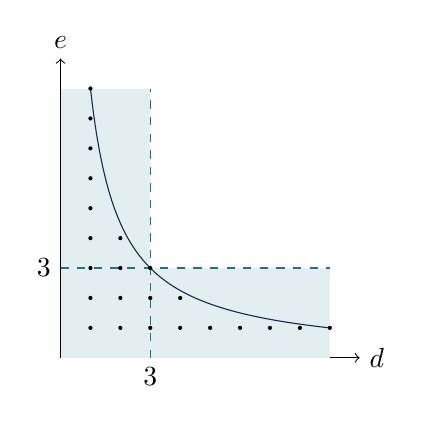
\begin{tikzpicture}[scale=.38]
\draw[->] (0,0)--(10,0) node[right]{$d$};\draw[->](0,0)--(0,10) node[above]{$e$};
\fill[teal!12](0,0)rectangle(3,9);\fill[teal!12](3,0)rectangle(9,3);
\draw[teal,dashed](3,0)--(3,9);\draw[teal,dashed](0,3)--(9,3);
\draw[navy,domain=1:9,samples=80]plot(\x,{9/\x});
\foreach \d in {1,...,9}{\foreach \e in {1,...,9}{\pgfmathtruncatemacro{\ok}{\d*\e<=9}\ifnum\ok=1\fill(\d,\e)circle(2pt);\fi}}
\node[below]at(3,0){$3$};\node[left]at(0,3){$3$};
\end{tikzpicture}
\end{column}
\begin{column}{.5\textwidth}
Here $x=9$. Each dot is a pair of positive integers $d,e$ with $de\le9$.

Count the pairs with $d\le3$, then those with $e\le3$. Every pair is counted, and the nine pairs with both coordinates at most $3$ are counted twice.

For general $x$, split at $\sqrt x$.
\end{column}\end{columns}
\end{frame}
\begin{frame}{The average order of $\tau(n)$}
Since $\tau(n)$ counts positive divisors,
\[\sum_{n\le x}\tau(n)=\sum_{de\le x}1
=2\sum_{d\le\sqrt x}\left\lfloor\frac xd\right\rfloor-\lfloor\sqrt x\rfloor^2.\]
Every pair has $d\le\sqrt x$ or $e\le\sqrt x$; the square is counted twice.

Dropping the floors in the sum costs $O(\sqrt x)$, and $\lfloor\sqrt x\rfloor^2=x+O(\sqrt x)$. The harmonic-sum estimate therefore gives
\[\sum_{n\le x}\tau(n)=x\log x+(2\gamma-1)x+O(\sqrt x).\]
\end{frame}
\begin{frame}{From $M(x)=o(x)$ to the PNT}
Subtracting our estimate for $\sum_{n\le x}\tau(n)$ from the one for $\sum_{n\le x}\log n$ gives
\[\sum_{n\le x}(\log n-\tau(n))=-2\gamma x+O(\sqrt x).\]
Too large! So put
\[g(n)=\log n-\tau(n)+2\gamma,\qquad G(x)=\sum_{n\le x}g(n).\]
Since $2\gamma\lfloor x\rfloor=2\gamma x+O(1)$, we have $G(x)=O(\sqrt x)$.

Recall $\sum_{d\mid n}\mu(d)\log(n/d)=\Lambda(n)$. What happens with $\tau$ in place of the logarithm?
\end{frame}
\begin{frame}{The convolution identity}
Expand $\tau(n/d)$ and sum on $e$ first:
\[\sum_{d\mid n}\mu(d)\tau(n/d)=\sum_{de\mid n}\mu(d)
=\sum_{e\mid n}\sum_{d\mid n/e}\mu(d)=\sum_{e\mid n}\ind_{n/e=1}=1.\]
Consequently
\[\sum_{dj=n}\mu(d)g(j)=\Lambda(n)-1+2\gamma\ind_{n=1}.\]
Summing, it remains to prove
\[\psi(x)-\lfloor x\rfloor+2\gamma=\sum_{dj\le x}\mu(d)g(j)=o(x).\]
\end{frame}
\begin{frame}{Using the hyperbola method again}
\small
Fix a positive integer $K$. For $x\ge K$, split according as $j\le K$ or $j>K$:
\[\sum_{dj\le x}\mu(d)g(j)=\sum_{j\le K}g(j)M(x/j)
+\sum_{d\le x/K}\mu(d)\bigl(G(x/d)-G(K)\bigr).\]
For each fixed $j$, $M(x/j)=o(x)$, so the first sum is $o_K(x)$.

In the second, $x/d\ge K$, and
\[|G(x/d)-G(K)|\ll\sqrt{x/d}+\sqrt K\ll\sqrt{x/d},\]
with constants independent of $K$. Its absolute value is bounded by a constant times
\[\sqrt x\sum_{d\le x/K}\frac1{\sqrt d}\le2\sqrt x\sqrt{x/K}=\frac{2x}{\sqrt K}.\]
\end{frame}
\begin{frame}{The prime number theorem}
For every fixed $K\ge1$,
\[\psi(x)-x=o_K(x)+O(x/\sqrt K).\]
Divide by $x$ and take the limsup:
\[\limsup_{x\to\infty}\left|\frac{\psi(x)}x-1\right|\le\frac C{\sqrt K}.\]
Since $K$ can be taken arbitrarily large, the limsup is zero. Thus
\[\boxed{\psi(x)\sim x.}\]
\end{frame}


% ---- sections/08-bonus ----
\section{BONUS}
\begin{frame}{BONUS: $\sum \mu(n)/n=0$}
We know $M(x)=o(x)$. First we prove a lemma:
\[R(x):=\sum_{d\le x}\mu(d)\left\{\frac xd\right\}=o(x).\]
Fix an integer $K>2$. We break the sum at $x/K$. Then
\[\left|\sum_{d\le x/K}\mu(d)\left\{\frac xd\right\}\right|\le\frac xK.\]
Now consider $x/K<d\le x$. I claim this part of the sum is $o(x)$!
\end{frame}
\begin{frame}{BONUS: partial summation}
\small
Put $a=x/K$. Partial summation gives
\[x\sum_{a<d\le x}\frac{\mu(d)}d=M(x)-KM(a)+x\int_a^x\frac{M(t)}{t^2}\dd t.\]
For $d>a$, the integer $\lfloor x/d\rfloor$ counts $1\le j\le K-1$ with $d\le x/j$. Thus
\[\sum_{a<d\le x}\mu(d)\left\lfloor\frac xd\right\rfloor
=\sum_{j=1}^{K-1}\bigl(M(x/j)-M(a)\bigr).\]
Subtracting the two identities gives
\[\sum_{x/K<d\le x}\mu(d)\left\{\frac xd\right\}
=x\int_{x/K}^x\frac{M(t)}{t^2}\dd t-\sum_{j=2}^K M(x/j).\]
\end{frame}
\begin{frame}{BONUS: the fractional-part sum is $o(x)$}
Divide the last identity by $x$. Each term $M(x/j)/x$ goes to zero, for $j=2,\ldots,K$. Also,
\[\left|\int_{x/K}^x\frac{M(t)}{t^2}\dd t\right|
\le\sup_{t\ge x/K}\frac{|M(t)|}t\int_{x/K}^x\frac{\dd t}t
=\log K\sup_{t\ge x/K}\frac{|M(t)|}t\longrightarrow0.\]
Therefore
\[|R(x)|\le\frac xK+o_K(x),\qquad
\limsup_{x\to\infty}\frac{|R(x)|}x\le\frac1K.\]
Take $K$ large. This proves $R(x)=o(x)$.
\end{frame}
\begin{frame}{BONUS: $\sum \mu(n)/n=0$}
We showed that
\begin{align*}
1&=\sum_{n\le x}\sum_{d\mid n}\mu(d)
=\sum_{d\le x}\mu(d)\left\lfloor\frac xd\right\rfloor\\
&=x\sum_{d\le x}\frac{\mu(d)}d-R(x).
\end{align*}
Rearranging,
\[\sum_{d\le x}\frac{\mu(d)}d=\frac1x+\frac{R(x)}x\longrightarrow0.\]
We win!
\[\boxed{\displaystyle\sum_{n=1}^\infty\frac{\mu(n)}n=0.}\]
\end{frame}


% ---- sections/09-references ----
\section{Course materials}
\begin{frame}{Course materials}
\small
\link{https://www.pollack-math.net/8440f26.html}{\textbf{MATH 8440, Fall 2026}}\\
University of Georgia. The course page has the dated lecture record and four assignments.

\link{https://www.pollack-math.net/8440f26/HW1.pdf}{Homework 1}\quad
\link{https://www.pollack-math.net/8440f26/HW2.pdf}{Homework 2}\quad
\link{https://www.pollack-math.net/8440f26/HW3.pdf}{Homework 3}\quad
\link{https://www.pollack-math.net/8440f26/HW4.pdf}{Homework 4}

\link{https://www.pollack-math.net/NABDofficial.pdf}{\textbf{Not Always Buried Deep}}\\
Paul Pollack, \emph{A Second Course in Elementary Number Theory}, AMS, 2009. Chapters 1, 3, and 4 accompany the lectures on infinitude, prime estimates, and progressions. The constant in Mertens' product is Theorem 3.17.

\link{https://www.pollack-math.net/8440f26/pnt-part-i.pdf}{\textbf{From M\"obius sums to the PNT}}\\
The course handout for the final sequence of lectures.
\end{frame}

% ---- sections/further-reading ----
\begin{frame}{Further reading}
\link{https://hexagonmath.org/2610.00545v1}{\textbf{The missing Lin(ni)k}}

Paul Pollack, Hexagon, 2026. An elementary proof of Linnik's theorem using Selberg's symmetry formulas and the exclusion of Siegel zeros.

\link{https://hexagonmath.org/2611.00636v1}{\textbf{Daboussi's elementary proof of the prime number theorem, reconsidered}}

Paul Pollack, Hexagon, 2026. A simplification of Daboussi's smooth-number argument for $M(x)=o(x)$, underlying the final part of these notes.

\link{\oaurl}{\textbf{Uniform exclusion of Landau--Siegel zeros}}

OpenAI, October 2026. The breakthrough excluding real zeros uniformly close to $1$ on the scale $1/\log m$.
\end{frame}


\end{document}
